\chapter{周期范畴}
\markboth{周期范畴}{周期范畴}

\begin{remark}[本章的外部依赖与阅读顺序]\label{rem:periodic_category_dependencies}
本章把前几章的结论提升到范畴层面，行文中因此会引用若干\textbf{排在其后}的章节中的定理。为使每一步都可验证，现将这些依赖集中列出；正文出现处均给出明确的交叉引用。
\begin{enumerate}[label=(\roman*)]
    \item \cref{thm:helmholtz}（「矢量分析」章）——亥姆霍兹分解；
    \item \cref{thm:noether_group_with_periodic_orbits}（「周期函数与具有周期轨道的群」章）——周期函数层面的诺特定理；
    \item \cref{prop:commensurability_periodicity_parallel}、\cref{thm:intercalation_error_bound_parallel}、\cref{thm:continued_fraction_best_approx_parallel}（「离散采样逼近、同余角与置闰」章）——可公度性平行命题、置闰误差有界与连分数最优性；
    \item \cref{thm:discrete_parseval_parallel}（「离散采样逼近」章）、\cref{thm:parseval_fourier}、\cref{thm:intercalation_dft_leakage}（「调和分析」章）——离散与连续帕塞瓦尔恒等式、DFT 泄露估计。
\end{enumerate}
\textbf{阅读建议}：本章的抽象结论可视为对已证具体结果的\textbf{形式化包装}，其证明中不出现新的实质数学内容。初读时可先跳过本章，待「调和分析」章之后再回读，则全部依赖已就位。
\end{remark}

\begin{remark}[本章定位]\label{rem:periodic_category_chapter_positioning}
周期范畴是周期数学的最高层统一理论。本章将前面各章建立的数学结构——具有周期轨道的群、周期函数、周期卷积、周期流形——统一纳入范畴论的语言。范畴论为周期数学提供了最抽象的表述框架，揭示了不同周期结构之间深层的结构同一性。

本章首先严格区分\textbf{算子}与\textbf{函子}这两个基本概念：算子是同一范畴内的自映射，函子是不同范畴之间的保结构映射。在此基础上，本章建立\textbf{相位函子}的完整理论：对任意周期 $T$ 和任意相位 $\theta \in [0, 2\pi)$，存在一个相位函子 $\Phi_{\theta, T}$，将平移周期范畴映射到自身。所有相位函子构成一个参数化的函子族。

本章的核心内容：
\begin{enumerate}[label=(\arabic*)]
    \item \textbf{算子与函子的严格区分}：算子（定义 \ref{def:operator}）与函子（定义 \ref{def:functor}）在作用域和结构保持性上的本质区别。
    \item \textbf{相位函子}：对任意周期 $T$ 和任意相位 $\theta$，相位函子 $\Phi_{\theta, T}$（定义 \ref{def:phase_functor_general}）实现周期结构的相位平移。
    \item \textbf{三种基本周期范畴}：平移周期范畴、缩放周期范畴、旋转周期范畴（定义 \ref{def:translation_periodic_category} 至 \ref{def:scaling_periodic_category}）。
    \item \textbf{函子作为范畴转换器}：对数函子实现缩放范畴到平移范畴的转换，傅里叶函子实现平移范畴到频域表示范畴的转换。
    \item \textbf{微分算子与积分算子的伴随性}：$\mathcal{D} \dashv \mathcal{I}$。
    \item \textbf{周期卷积作为双函子}：周期卷积是周期范畴上的双函子。
    \item \textbf{观察者作为函子}：观察者将时间系统和空间系统的周期结构投影为可观测痕迹。
\end{enumerate}

\textbf{本章七主题导引}：平移——平移周期范畴 $\mathcal{C}_{\text{trans}}$ 与微分算子 $\mathcal{D}$（$0$-对称）；缩放——缩放周期范畴与对数函子/指数函子（$1$-对称）；旋转——旋转周期范畴与相位函子（$i$-对称）；守恒——伴随算子的守恒条件（$\mathcal{I}\circ\mathcal{D}\cong\operatorname{id}$ 要求积分为零，对应角动量守恒）；对称——自然同构与伴随对偶 $\mathcal{D}\dashv\mathcal{I}$；闭合——微分-积分算子的互逆闭合、周期卷积双函子的闭合格；周期——周期流形的范畴表述与相位函子的参数化。
\end{remark}

\begin{figure}[htbp]
\centering
\begin{tikzpicture}[
  font=\small,
  box/.style={draw, rounded corners, fill=blue!8, minimum width=2.6cm, minimum height=0.8cm, align=center},
  sub/.style={draw, rounded corners, fill=green!10, minimum width=2.4cm, minimum height=0.7cm, align=center, font=\footnotesize},
  arr/.style={->, thick, >=stealth}
]
  \node[box] (cat) {范畴论基础\\范畴/函子/自然变换};
  \node[box, right=1.0cm of cat] (phase) {相位函子\\$\Phi_{\theta,T}$};
  \node[box, right=1.0cm of phase] (three) {三种周期范畴\\平移/缩放/旋转};
  \node[sub, below=1.0cm of cat] (diff) {微分-积分伴随\\$\mathcal D\dashv\mathcal I$};
  \node[sub, below=1.0cm of phase] (conv) {周期卷积双函子\\$\circledast$};
  \node[sub, below=1.0cm of three] (obs) {观察者函子\\$\mathcal P$};
  \node[box, fill=orange!12, below=1.0cm of $(diff)!0.5!(obs)$] (unify) {周期数学的范畴论统一};
  \draw[arr] (cat) -- (phase);
  \draw[arr] (phase) -- (three);
  \draw[arr] (cat) -- (diff);
  \draw[arr] (phase) -- (conv);
  \draw[arr] (three) -- (obs);
  \draw[arr] (diff) -- (unify);
  \draw[arr] (conv) -- (unify);
  \draw[arr] (obs) -- (unify);
\end{tikzpicture}
\caption{本章结构总览：从范畴论基础出发，经相位函子与三种周期范畴，到微分-积分伴随、周期卷积双函子与观察者函子，最终统一于周期数学的范畴论框架。}
\label{fig:periodic_category_overview}
\end{figure}

\section{范畴论基础}\label{sec:category_theory_basics}

\begin{definition}[范畴]\label{def:category}
一个\textbf{范畴} $\mathcal{C}$ 由以下数据构成：
\begin{enumerate}[label=(\roman*)]
    \item 一个\textbf{对象}的类 $\operatorname{Ob}(\mathcal{C})$。
    \item 对任意两个对象 $A, B \in \operatorname{Ob}(\mathcal{C})$，有一个\textbf{态射}的集合 $\operatorname{Hom}_{\mathcal{C}}(A, B)$。
    \item 对任意对象 $A$，有一个\textbf{恒等态射} $\operatorname{id}_A \in \operatorname{Hom}_{\mathcal{C}}(A, A)$。
    \item 对任意三个对象 $A, B, C$，有一个\textbf{复合}运算 $\circ: \operatorname{Hom}_{\mathcal{C}}(B, C) \times \operatorname{Hom}_{\mathcal{C}}(A, B) \to \operatorname{Hom}_{\mathcal{C}}(A, C)$。
\end{enumerate}
满足以下公理：
\begin{itemize}
    \item \textbf{结合律}：对任意 $f: A \to B, g: B \to C, h: C \to D$，有 $h \circ (g \circ f) = (h \circ g) \circ f$。
    \item \textbf{单位律}：对任意 $f: A \to B$，有 $f \circ \operatorname{id}_A = f = \operatorname{id}_B \circ f$。
\end{itemize}
\end{definition}

\begin{example}[周期数学中的范畴实例]\label{ex:category_instances}
\begin{itemize}
    \item \textbf{集合范畴} $\mathbf{Set}$：对象为集合，态射为函数。
    \item \textbf{向量空间范畴} $\mathbf{Vect}_{\mathbb{C}}$：对象为复向量空间，态射为线性映射。
    \item \textbf{群范畴} $\mathbf{Grp}$：对象为群，态射为群同态。
    \item \textbf{拓扑空间范畴} $\mathbf{Top}$：对象为拓扑空间，态射为连续映射。
    \item \textbf{光滑流形范畴} $\mathbf{Man}$：对象为光滑流形，态射为光滑映射。
\end{itemize}
\end{example}

\begin{figure}[htbp]
\centering
\begin{tikzpicture}[
  font=\small,
  obj/.style={circle, draw, fill=blue!8, minimum size=0.8cm, inner sep=2pt},
  arr/.style={->, thick, >=stealth}
]
  \node[obj] (A) at (0,0) {$A$};
  \node[obj] (B) at (3,0) {$B$};
  \node[obj] (C) at (6,0) {$C$};
  \draw[arr] (A) -- node[above, font=\footnotesize]{$f$} (B);
  \draw[arr] (B) -- node[above, font=\footnotesize]{$g$} (C);
  \draw[arr, bend left=25] (A) to node[below, font=\footnotesize]{$g\circ f$} (C);
  \node[font=\footnotesize] at (3,-1.2) {结合律：$h\circ(g\circ f)=(h\circ g)\circ f$};
\end{tikzpicture}
\caption{范畴的基本结构：对象、态射与复合。}
\label{fig:category_structure}
\end{figure}

\section{算子与函子}\label{sec:operator_vs_functor}

\begin{definition}[算子]\label{def:operator}
设 $\mathcal{C}$ 为范畴。$\mathcal{C}$ 上的一个\textbf{算子}是一个映射 $T: \operatorname{Ob}(\mathcal{C}) \to \operatorname{Ob}(\mathcal{C})$，满足对任意态射 $f: A \to B$，存在态射 $T(f): T(A) \to T(B)$，且 $T(\operatorname{id}_A) = \operatorname{id}_{T(A)}$，$T(g \circ f) = T(g) \circ T(f)$。

换句话说，算子是\textbf{范畴到自身的函子}（自函子），即 $T: \mathcal{C} \to \mathcal{C}$。算子保持范畴的内部结构，不改变对象所在的范畴。

在周期数学中，微分算子 $\mathcal{D}$、积分算子 $\mathcal{I}$ 都是平移周期范畴 $\mathcal{C}_{\text{trans}}$ 上的算子（自函子）。
\end{definition}

\begin{definition}[函子]\label{def:functor}
设 $\mathcal{C}$ 和 $\mathcal{D}$ 为两个范畴。一个\textbf{函子} $F: \mathcal{C} \to \mathcal{D}$ 由以下数据构成：
\begin{enumerate}[label=(\roman*)]
    \item 对每个对象 $A \in \operatorname{Ob}(\mathcal{C})$，有一个对象 $F(A) \in \operatorname{Ob}(\mathcal{D})$。
    \item 对每个态射 $f: A \to B$（在 $\mathcal{C}$ 中），有一个态射 $F(f): F(A) \to F(B)$（在 $\mathcal{D}$ 中）。
\end{enumerate}
满足 $F(\operatorname{id}_A) = \operatorname{id}_{F(A)}$ 和 $F(g \circ f) = F(g) \circ F(f)$。

若 $F$ 反转态射方向（即 $F(f): F(B) \to F(A)$），则称 $F$ 为\textbf{反变函子}。
\end{definition}

\begin{remark}[算子与函子的区别]\label{rem:operator_vs_functor}
算子与函子的本质区别在于\textbf{作用域}：
\begin{itemize}
    \item \textbf{算子}（自函子）$T: \mathcal{C} \to \mathcal{C}$ 将范畴映射到\textbf{自身}，保持对象和态射的类型不变。微分算子 $\mathcal{D}$ 将周期函数映射为周期函数，将周期态射映射为周期态射——周期结构在算子作用下保持不变。
    \item \textbf{函子} $F: \mathcal{C} \to \mathcal{D}$ 将范畴映射到\textbf{另一个范畴}，改变对象和态射的类型。傅里叶函子 $\mathcal{F}: \mathcal{C}_{\text{trans}} \to \mathbf{Vect}_{\mathbb{C}}$ 将周期函数映射为傅里叶系数向量，将周期态射映射为线性映射——周期结构被“编码”为频域中的代数结构。
\end{itemize}
从周期数学的视角看：算子保持周期类型（平移周期函数经微分后仍是平移周期函数），函子转换周期类型（平移周期函数经傅里叶变换后成为频域中的离散序列）。
\end{remark}

\begin{figure}[htbp]
\centering
\begin{tikzpicture}[
  font=\small,
  cat/.style={draw, rounded corners, fill=blue!8, minimum width=2.8cm, minimum height=0.9cm, align=center},
  arr/.style={->, thick, >=stealth}
]
  % 算子
  \node[cat] (C1) at (0,0) {$\mathcal C$};
  \draw[arr] (C1) to[loop above] node[above, font=\footnotesize]{算子 $T$} (C1);
  \node[font=\footnotesize] at (0,-1.0) {范畴到自身};
  % 函子
  \node[cat] (C2) at (5,0) {$\mathcal C$};
  \node[cat, fill=green!10] (D2) at (9,0) {$\mathcal D$};
  \draw[arr] (C2) -- node[above, font=\footnotesize]{函子 $F$} (D2);
  \node[font=\footnotesize] at (7,-1.0) {范畴到范畴};
\end{tikzpicture}
\caption{算子（自函子）与函子的作用域对比：算子不改变范畴，函子跨范畴映射。}
\label{fig:operator_vs_functor}
\end{figure}

\section{相位函子}\label{sec:phase_functor}

\begin{definition}[相位函子]\label{def:phase_functor_general}
设 $\mathcal{C}_{\text{trans}}$ 为平移周期范畴。对任意周期 $T > 0$ 和任意相位 $\theta \in [0, 2\pi)$，定义\textbf{相位函子} $\Phi_{\theta, T}: \mathcal{C}_{\text{trans}} \to \mathcal{C}_{\text{trans}}$ 为：
\[
\Phi_{\theta, T}(f)(t) = e^{i\theta} \cdot f\!\left( t - \frac{\theta T}{2\pi} \right).
\]
即相位函子将周期函数 $f$ 时间平移 $\frac{\theta T}{2\pi}$（相位 $\theta$ 对应的时间偏移），并乘以相位因子 $e^{i\theta}$。

相位函子族 $\{\Phi_{\theta, T}\}_{\theta \in [0, 2\pi), T > 0}$ 的参数空间是 $S^1 \times \mathbb{R}^+$。
\end{definition}

\begin{proposition}[相位函子的基本性质]\label{prop:phase_functor_properties}
相位函子 $\Phi_{\theta, T}$ 满足以下性质：
\begin{enumerate}[label=(\roman*)]
    \item \textbf{函子性}：$\Phi_{\theta, T}$ 是 $\mathcal{C}_{\text{trans}}$ 上的自函子（算子）。
    \item \textbf{保持周期}：$\operatorname{Group}_{\mathrm{period}}(\Phi_{\theta, T}(f)) = \operatorname{Group}_{\mathrm{period}}(f)$——相位函子不改变周期。
    \item \textbf{复合律}：$\Phi_{\theta_1, T} \circ \Phi_{\theta_2, T} = \Phi_{\theta_1 + \theta_2, T}$（模 $2\pi$）。
    \item \textbf{恒等元}：$\Phi_{0, T} = \operatorname{id}_{\mathcal{C}_{\text{trans}}}$（纯时间平移，无相位因子）。
    \item \textbf{逆元}：$\Phi_{\theta, T}^{-1} = \Phi_{-\theta, T} = \Phi_{2\pi - \theta, T}$。
    \item \textbf{幺正性}：$\|\Phi_{\theta, T}(f)\| = \|f\|$（$L^2$ 范数保持不变）。
\end{enumerate}
\end{proposition}

\begin{proof}
(i) 对任意周期态射 $h: f \to g$，$\Phi_{\theta, T}(h) = h$（因为相位函子只平移时间参数，不改变态射的线性结构）。恒等态射和复合的保持由定义直接验证。

(ii) 时间平移不改变周期：$f(t + T) = f(t)$ 蕴含 $f(t - \frac{\theta T}{2\pi} + T) = f(t - \frac{\theta T}{2\pi})$。乘以 $e^{i\theta}$ 也不改变周期。

(iii)
\[
\Phi_{\theta_1, T}(\Phi_{\theta_2, T}(f))(t) = e^{i\theta_1} \Phi_{\theta_2, T}(f)\!\left( t - \tfrac{\theta_1 T}{2\pi} \right) = e^{i\theta_1} e^{i\theta_2} f\!\left( t - \tfrac{\theta_1 T}{2\pi} - \tfrac{\theta_2 T}{2\pi} \right) = \Phi_{\theta_1 + \theta_2, T}(f)(t).
\]

(iv) $\Phi_{0, T}(f)(t) = e^{i0} f(t - 0) = f(t)$。

(v) 由 (iii)，$\Phi_{\theta, T} \circ \Phi_{-\theta, T} = \Phi_{0, T} = \operatorname{id}$。

(vi) $\|\Phi_{\theta, T}(f)\|^2 = \frac{1}{T}\int_0^T |e^{i\theta} f(t - \frac{\theta T}{2\pi})|^2 dt = \frac{1}{T}\int_0^T |f(t)|^2 dt = \|f\|^2$（时间平移和乘以单位复数均保持 $L^2$ 范数）。
\end{proof}

\begin{theorem}[相位函子族的群结构]\label{thm:phase_functor_group}
对固定周期 $T > 0$，相位函子族 $\{\Phi_{\theta, T}\}_{\theta \in [0, 2\pi)}$ 在函子复合下构成一个群，同构于圆群 $U(1)$：
\[
\{\Phi_{\theta, T}\}_{\theta \in [0, 2\pi)} \cong U(1) \cong S^1.
\]
\end{theorem}

\begin{proof}
由命题 \ref{prop:phase_functor_properties} 的 (iii)(iv)(v)，集合 $\{\Phi_{\theta, T}\}$ 在复合下封闭，含恒等元 $\Phi_{0, T}$，每个元素有逆元 $\Phi_{-\theta, T}$。结合律由函数复合的结合律给出。映射 $\theta \mapsto \Phi_{\theta, T}$ 是群同构：$\Phi_{\theta_1 + \theta_2} = \Phi_{\theta_1} \circ \Phi_{\theta_2}$（模 $2\pi$），$\Phi_0 = \operatorname{id}$，$\Phi_{-\theta} = \Phi_\theta^{-1}$。故相位函子族同构于 $U(1)$。
\end{proof}

\begin{corollary}[所有相位的函子性]\label{cor:all_phases_functorial}
对任意周期 $T > 0$ 和任意相位 $\theta \in [0, 2\pi)$，$\Phi_{\theta, T}$ 都是 $\mathcal{C}_{\text{trans}}$ 上的函子（算子）。因此，\textbf{所有周期的任意相位都可以作为函子}——相位不再是函数的附加参数，而是范畴上的结构保持映射。
\end{corollary}

\begin{proof}
由定理 \ref{thm:phase_functor_group}，每个 $\Phi_{\theta, T}$ 是群 $U(1)$ 中的元素，因而是可逆函子（自同构函子）。函子性由命题 \ref{prop:phase_functor_properties} (i) 保证。
\end{proof}

\begin{remark}[相位函子与离散相位算子]\label{rem:phase_functor_discrete}
当相位取离散值 $\theta_k = 2\pi k/T$（$k = 0, 1, \dots, T-1$）时，相位函子族 $\{\Phi_{\theta_k, T}\}_{k=0}^{T-1}$ 同构于循环群 $C_T \cong \mathbb{Z}_T$。这是“周期函数与具有周期轨道的群”章中离散相位算子 $\mathcal{O}_k^{(T)} = e^{i 2\pi k / T}$（定义 \ref{def:discrete_phase_operator}）的函子化表述。连续相位函子族 $U(1)$ 是离散相位算子族 $C_T$ 的连续极限（$T \to \infty$）。
\end{remark}

\begin{example}[相位函子的具体作用]\label{ex:phase_functor_action}
取 $T = 2\pi$，$f(t) = \sin t$。对相位 $\theta = \pi/2$：
\[
\Phi_{\pi/2, 2\pi}(f)(t) = e^{i\pi/2} \sin\!\left( t - \frac{\pi/2 \cdot 2\pi}{2\pi} \right) = i \sin\!\left( t - \frac{\pi}{2} \right) = -i \cos t.
\]
即相位函子 $\Phi_{\pi/2, 2\pi}$ 将正弦函数映射为余弦函数（乘以 $-i$）。这正是傅里叶分析中相位移位的标准操作。

对相位 $\theta = \pi$：
\[
\Phi_{\pi, 2\pi}(f)(t) = e^{i\pi} \sin(t - \pi) = -\sin(t - \pi) = \sin t = f(t).
\]
（注意 $\sin(t - \pi) = -\sin t$，故 $e^{i\pi}\sin(t-\pi) = (-1)(-\sin t) = \sin t$。）即相位 $\pi$ 的函子对正弦函数是恒等映射（因为正弦函数在时间平移半周期后变号，乘以 $-1$ 后恢复原状）。
\end{example}

\begin{figure}[htbp]
\centering
\begin{tikzpicture}[scale=0.9]

  \draw[->, thick, >=stealth] (-2,0) -- (2,0);
  \draw[->, thick, >=stealth] (0,-2) -- (0,2);

  \draw[thick, blue] (0,0) circle (1.5);

  \foreach \a in {0,45,90,180,270} {
    \node[circle, fill, red, inner sep=1.5pt] at (\a:1.5) {};
  }

  \node[font=\footnotesize, xshift=1cm] at (0:1.9) {$\theta=0$};
  \node[font=\footnotesize, yshift=0.5cm] at (90:1.9) {$\theta=\pi/2$};
  \node[font=\footnotesize, xshift=-1cm] at (180:1.9) {$\theta=\pi$};
  \node[font=\footnotesize, yshift=-0.5cm] at (270:1.9) {$\theta=3\pi/2$};

  \draw[->, thick, orange, >=stealth] (1.0,0.3) arc (15:75:1.1);
  \node[orange, font=\footnotesize, xshift=0.5cm] at (1.6,0.8) {旋转};
  \node[yshift=-1cm] at (0,-2.5) {$U(1)$：相位函子族};
\end{tikzpicture}
\caption{相位函子族构成圆群 $U(1)$：相位参数 $\theta$ 在单位圆上连续取值。}
\label{fig:phase_functor_U1}
\end{figure}

\section{变换与演化}\label{sec:transformation_evolution}

在范畴论中，结构的变化由两类基本机制描述：\textbf{变换}（自然变换）刻画函子之间的比较，\textbf{演化}（伴随函子）刻画范畴之间的相互生成与遗忘。本节建立这两类机制，并说明它们如何编码周期结构的生灭。

\begin{definition}[自然变换]\label{def:natural_transformation}
设 $F, G: \mathcal{C} \to \mathcal{D}$ 为两个平行函子。一个\textbf{自然变换} $\eta: F \Rightarrow G$ 由一族态射 $\{\eta_A: F(A) \to G(A)\}_{A \in \operatorname{Ob}(\mathcal{C})}$ 构成，使得对任意 $f: A \to B$（在 $\mathcal{C}$ 中），下图交换：
\[
\begin{tikzcd}
F(A) \arrow[r, "F(f)"] \arrow[d, "\eta_A"'] & F(B) \arrow[d, "\eta_B"] \\
G(A) \arrow[r, "G(f)"'] & G(B)
\end{tikzcd}
\]
即 $\eta_B \circ F(f) = G(f) \circ \eta_A$。
\end{definition}

\begin{definition}[伴随函子]\label{def:adjoint_functor}
设 $F: \mathcal{C} \to \mathcal{D}$ 和 $G: \mathcal{D} \to \mathcal{C}$ 为两个函子。称 $F$ 是 $G$ 的\textbf{左伴随}（或 $G$ 是 $F$ 的\textbf{右伴随}），记作 $F \dashv G$，如果存在自然同构
\[
\operatorname{Hom}_{\mathcal{D}}(F(A), B) \cong \operatorname{Hom}_{\mathcal{C}}(A, G(B)),
\]
该同构对 $A \in \operatorname{Ob}(\mathcal{C})$ 和 $B \in \operatorname{Ob}(\mathcal{D})$ 自然。
\end{definition}

\begin{remark}[伴随函子与周期生灭]\label{rem:adjunction_periodic_lifecycle}
在周期数学中，伴随函子对 $F \dashv G$ 具有深刻的周期论含义：$F$ 是“生成”方向（对称破缺，周期结构的涌现），$G$ 是“遗忘”方向（周期结构的退化）。伴随对 $(F, G)$ 构成了周期结构生灭的范畴论模型——生成（伴随函子的单位 $\eta$）、演化（态射的复合）、消亡（伴随函子的余单位 $\varepsilon$ 的退化）。

从守恒律的视角看，伴随对 $F \dashv G$ 的\textbf{单位} $\eta: \operatorname{id}_{\mathcal{C}} \Rightarrow G \circ F$ 编码了“从无周期到有周期”的生成过程（守恒律的建立），而\textbf{余单位} $\varepsilon: F \circ G \Rightarrow \operatorname{id}_{\mathcal{D}}$ 编码了“从有周期到无周期”的消亡过程（守恒律的破缺）。
\end{remark}

\begin{figure}[htbp]
\centering
\begin{tikzcd}[row sep=large, column sep=large]
\mathcal{C} \arrow[r, bend left=25, "F"] & \mathcal{D} \arrow[l, bend left=25, "G"]
\end{tikzcd}
\vspace{0.3cm}
\begin{tikzpicture}[font=\footnotesize]
  \node at (0,0) {$\operatorname{Hom}_{\mathcal D}(F(A),B)\cong\operatorname{Hom}_{\mathcal C}(A,G(B))$};
  \node at (0,-0.6) {$F\dashv G$：左伴随（生成） $\dashv$ 右伴随（遗忘）};
\end{tikzpicture}
\caption{伴随函子对 $F\dashv G$ 与 Hom 集自然同构。}
\label{fig:adjoint_functor}
\end{figure}

\section{周期范畴的基本构造}\label{sec:periodic_category_basic}

\subsection{周期对象与周期态射}

\begin{definition}[周期对象]\label{def:periodic_object}
设 $\mathcal{C}$ 为范畴，$G$ 为群。$\mathcal{C}$ 中的一个\textbf{$G$-周期对象}是一个二元组 $(X, \rho)$，其中 $X \in \operatorname{Ob}(\mathcal{C})$，$\rho: G \to \operatorname{Aut}_{\mathcal{C}}(X)$ 是 $G$ 在 $X$ 上的群作用（即 $\rho(g): X \to X$ 是 $\mathcal{C}$ 中的自同构，且 $\rho(gh) = \rho(g) \circ \rho(h)$）。

在周期数学中，$G$ 通常取为平移群 $\mathbb{R}$、缩放群 $\mathbb{R}^+$ 或旋转群 $U(1)$。
\end{definition}

\begin{proposition}[周期对象与守恒律]\label{prop:periodic_object_conservation}
$G$-周期对象 $(X, \rho)$ 的群作用 $\rho$ 蕴含了 $X$ 上的守恒结构：对任意 $g \in G$，$\rho(g)$ 是 $X$ 的自同构，保持 $X$ 的所有范畴论结构不变。当 $G$ 为连续李群时，由诺特定理，$G$ 的每个单参数子群对应 $X$ 上的一个守恒量。具体而言：
\begin{enumerate}[label=(\roman*)]
    \item 若 $G = \mathbb{R}$（平移群，$0$-对称），守恒量为动量/能量。
    \item 若 $G = U(1)$（旋转群，$i$-对称），守恒量为角动量。
    \item 若 $G = \mathbb{R}^+$（缩放群，$1$-对称），守恒量为标度荷。
\end{enumerate}
\end{proposition}

\begin{proof}
分三步，并标明每一步的性质。

\textbf{第一步（定义的展开，不含额外内容）}。按定义 \ref{def:periodic_object}，$\rho$ 是群同态 $G \to \operatorname{Aut}_{\mathcal{C}}(X)$，即每个 $\rho(g)$ 都是 $\mathcal{C}$ 中 $X$ 的自同构。自同构按定义保持态射的复合与恒等态射，故保持 $X$ 的一切范畴结构。这一步只是把“自同构”的定义重述一遍，因此它说明的是\textbf{结构不变}，尚未给出任何守恒量。

\textbf{第二步（守恒量的来源）}。守恒量来自具体层面的定理：由 \cref{thm:noether_group_with_periodic_orbits}，对连续李群 $G$ 的每个单参数子群 $\{g_s\}_{s \in \mathbb{R}}$，作用族 $\rho(g_s)$ 生成一个守恒荷。分别取
\[
\begin{aligned}
G = \mathbb{R} \;\Rightarrow\; &\text{平移荷（能量／动量，对称中心 } 0\text{）},\\
G = U(1) \;\Rightarrow\; &\text{旋转荷（角动量，对称中心 } i\text{）},\\
G = \mathbb{R}^+ \;\Rightarrow\; &\text{缩放荷（标度荷，对称中心 } 1\text{）}.
\end{aligned}
\]
即命题所列三条。

\textbf{第三步（守恒量集的刻画）}。对象 $(X, \rho)$ 的守恒量集合是全部单参数子群所对应荷的并集。当 $G$ 取 $\mathbb{R}$、$U(1)$、$\mathbb{R}^+$ 时，其单参数子群族分别为平移族、旋转族、缩放族，故三条逐一成立。证毕。

\textbf{依赖说明}：第二步用到 \cref{thm:noether_group_with_periodic_orbits}，该定理位于「周期函数与具有周期轨道的群」章，在本章之后；见本章开头的依赖声明 \cref{rem:periodic_category_dependencies}。
\end{proof}

\begin{definition}[周期态射]\label{def:periodic_morphism}
设 $(X, \rho)$ 和 $(Y, \sigma)$ 为 $\mathcal{C}$ 中两个 $G$-周期对象。一个\textbf{$G$-等变态射}（或\textbf{周期态射}）$f: X \to Y$ 满足对任意 $g \in G$，
\[
f \circ \rho(g) = \sigma(g) \circ f.
\]
即 $f$ 与群作用交换——$f$ 保持周期结构。全体 $G$-周期对象和 $G$-等变态射构成\textbf{周期范畴} $\mathcal{C}^G$。
\end{definition}

\begin{theorem}[周期范畴的守恒律保持]\label{thm:periodic_category_conservation}
设 $\mathcal{C}^G$ 为 $G$-周期范畴。则：
\begin{enumerate}[label=(\roman*)]
    \item $\mathcal{C}^G$ 中的每个对象 $(X, \rho)$ 携带 $G$ 的守恒量（由诺特定理给出）。
    \item $\mathcal{C}^G$ 中的每个周期态射 $f: (X, \rho) \to (Y, \sigma)$ 保持守恒量。
    \item $\mathcal{C}^G$ 中的同构类对应于具有相同守恒量结构的周期对象。
\end{enumerate}
\end{theorem}

\begin{proof}
(i) 由命题 \ref{prop:periodic_object_conservation} 直接得出。(ii) 周期态射 $f$ 与群作用交换：$f \circ \rho(g) = \sigma(g) \circ f$。对单参数子群求导，得 $f$ 将 $X$ 的诺特荷映射为 $Y$ 的诺特荷。(iii) 同构的周期对象具有同构的群作用和同构的守恒量空间。
\end{proof}

\begin{figure}[htbp]
\centering
\begin{tikzcd}[row sep=large, column sep=large]
X \arrow[r, "\rho(g)"] \arrow[d, "f"'] & X \arrow[d, "f"] \\
Y \arrow[r, "\sigma(g)"'] & Y
\end{tikzcd}
\caption{周期态射的等变性条件：$f\circ\rho(g)=\sigma(g)\circ f$。}
\label{fig:periodic_morphism}
\end{figure}

\subsection{三种基本周期范畴}

\begin{figure}[htbp]
\centering
\begin{tikzpicture}[>=stealth,
  cat/.style={draw, rounded corners, align=center, font=\small, inner sep=6pt}]
  \node[cat, fill=blue!8, minimum width=3.0cm] (A) at (0,0) {平移周期范畴\\[2pt]$\mathcal{C}_{\text{trans}}$};
  \node[cat, fill=green!10, minimum width=3.0cm] (B) at (5.0,0) {缩放周期范畴\\[2pt]$\mathcal{C}_{\text{scale}}$};
  \node[cat, fill=red!8, minimum width=3.0cm] (C) at (10.0,0) {旋转周期范畴\\[2pt]$\mathcal{C}_{\text{rot}}$};
  \draw[->,thick] (A) to[bend left=20] node[above,font=\footnotesize]{对数函子 $\mathcal{L}$} (B);
  \draw[->,thick] (B) to[bend left=20] node[below,font=\footnotesize,yshift=-0.3cm]{指数函子 $\mathcal{E}$} (A);
  \draw[->,thick] (B) to[bend left=20] node[above,font=\footnotesize]{单位圆限制 $|\lambda|=1$} (C);
  \draw[->,thick] (C) to[bend left=20] node[below,font=\footnotesize]{投影} (A);
  \node[font=\footnotesize] at (5.0,-2.0) {三类范畴之间以函子相互转换，而不是彼此等同};
\end{tikzpicture}
\caption{三种基本周期范畴及其转换函子。平移、缩放、旋转三类生成变换各对应一个周期范畴。对数函子把乘法型（缩放）结构化为加法型（平移）结构，其逆为指数函子；单位圆限制把缩放范畴中的单位模子范畴分离出来，得到旋转范畴；投影把旋转范畴送回平移范畴。此图同时说明：三类范畴并非彼此等同，而是由函子相互转换——这正是本章采用范畴论语言的理由。}
\label{fig:three_periodic_categories}
\end{figure}

\begin{definition}[平移周期范畴]\label{def:translation_periodic_category}
设 $G = \mathbb{R}$ 为平移群（加法群）。\textbf{平移周期范畴} $\mathcal{C}_{\text{trans}}$ 的对象为带有 $\mathbb{R}$-作用的周期对象——即平移周期函数 $f: \mathbb{R} \to \mathbb{C}$ 满足 $f(t+T) = f(t)$。态射为与平移作用交换的线性映射。
\end{definition}

\begin{definition}[旋转周期范畴]\label{def:rotation_periodic_category}
设 $G = U(1)$ 为旋转群。\textbf{旋转周期范畴} $\mathcal{C}_{\text{rot}}$ 的对象为带有 $U(1)$-作用的周期对象——即旋转周期函数 $f: \mathbb{C} \to \mathbb{C}$ 满足 $f(e^{i\theta}z) = f(z)$。态射为与旋转作用交换的线性映射。
\end{definition}

\begin{definition}[缩放周期范畴]\label{def:scaling_periodic_category}
设 $G = \mathbb{R}^+$ 为缩放群（乘法群）。\textbf{缩放周期范畴} $\mathcal{C}_{\text{scal}}$ 的对象为带有 $\mathbb{R}^+$-作用的周期对象——即缩放周期函数 $f: \mathbb{R}^+ \to \mathbb{C}$ 满足 $f(qx) = f(x)$。态射为与缩放作用交换的线性映射。
\end{definition}

\begin{lemma}[单周转圆对象之间的态射]\label{ch13_hom_frequency_lemma}
设 $\mathcal{C}_{\text{trans}}$ 为平移周期范畴，$f(t) = A\, e^{i(\omega_1 t + \varphi)}$，$g(t) = B\, e^{i(\omega_2 t + \psi)}$ 为其中两个单周转圆对象（$A, B > 0$，$\omega_1, \omega_2 \neq 0$）。则
\begin{enumerate}[label=(\roman*)]
    \item 若 $\omega_1 \neq \omega_2$，则 $\operatorname{Hom}_{\mathcal{C}_{\text{trans}}}(f, g) = \{0\}$；
    \item 若 $\omega_1 = \omega_2 = \omega$，则
    \[
    \operatorname{Hom}_{\mathcal{C}_{\text{trans}}}(f, g) = \Big\{ c \cdot \tfrac{B}{A}\, e^{i(\psi - \varphi)} : c \in \mathbb{C} \Big\}.
    \]
\end{enumerate}
\end{lemma}

\begin{proof}
平移群在单周转圆上的作用是标量乘法：$\rho_s(f)(t) = f(t+s) = e^{i\omega_1 s} f(t)$。$f$ 张成的子空间是一维的，故任何态射 $\lambda: f \to g$ 是标量乘法且必须满足 $\lambda f = c\, g$（$c \in \mathbb{C}$），即
\[
\lambda A e^{i\varphi} e^{i\omega_1 t} = c B e^{i\psi} e^{i\omega_2 t} \qquad (\forall t).
\]
(i) 若 $\omega_1 \neq \omega_2$：在 $t = 0$ 处取值得 $\lambda A e^{i\varphi} = c B e^{i\psi}$；再对 $t$ 求导后在 $t = 0$ 处取值得 $\lambda A e^{i\varphi} \omega_1 = c B e^{i\psi} \omega_2$。两式相除得 $\omega_1 = \omega_2$，矛盾，故 $\lambda = 0$、$c = 0$，即 $\operatorname{Hom}(f, g) = \{0\}$。
(ii) 若 $\omega_1 = \omega_2 = \omega$：上式化为 $\lambda A e^{i\varphi} = c B e^{i\psi}$，故 $\lambda = c\,(B/A)\,e^{i(\psi-\varphi)}$，$c$ 任意。等变性自动成立。
\end{proof}

\begin{example}[单周转圆态射集的具体计算]\label{ch13_hom_set_example}
取三个单周转圆对象：
\[
f(t) = 3 e^{i(2t + \pi/6)}, \qquad g(t) = 2 e^{i(3t - \pi/4)}, \qquad h(t) = 5 e^{i(2t + \pi/3)}.
\]
(i) $\omega_f = 2 \neq 3 = \omega_g$，由引理 \ref{ch13_hom_frequency_lemma} (i)，$\operatorname{Hom}(f, g) = \{0\}$。
(ii) $\omega_f = \omega_h = 2$，由引理 \ref{ch13_hom_frequency_lemma} (ii)，
\[
\operatorname{Hom}(f, h) = \Big\{ c \cdot \tfrac{5}{3}\, e^{i(\pi/3 - \pi/6)} : c \in \mathbb{C} \Big\} = \Big\{ c \cdot \tfrac{5}{3}\, e^{i\pi/6} : c \in \mathbb{C} \Big\}.
\]
取 $c = 1$ 得标准态射 $\lambda = \tfrac{5}{3} e^{i\pi/6}$，验证 $\lambda f(t) = \tfrac{5}{3} e^{i\pi/6} \cdot 3 e^{i(2t + \pi/6)} = 5 e^{i(2t + \pi/3)} = h(t)$。
(iii) 复合保持：再取 $k(t) = 4 e^{i 2t}$。$h \to k$ 的标准态射为 $\mu = \tfrac{4}{5} e^{-i\pi/3}$。$f \to k$ 的标准态射为 $\nu = \tfrac{4}{3} e^{-i\pi/6}$；复合 $\mu \circ \lambda = \tfrac{4}{5} e^{-i\pi/3} \cdot \tfrac{5}{3} e^{i\pi/6} = \tfrac{4}{3} e^{-i\pi/6} = \nu$。
\end{example}

\begin{remark}[振幅与相位不是平移周期范畴的不变量]\label{ch13_amplitude_phase_remark}
引理 \ref{ch13_hom_frequency_lemma} 与例 \ref{ch13_hom_set_example} 揭示了一个范畴论事实：在 $\mathcal{C}_{\text{trans}}$ 中，同频率的单周转圆对象彼此同构（任意 $c \neq 0$ 的标量态射都是同构），振幅 $A$ 与相位 $\varphi$ 并不进入同构不变量——它们被态射空间“吸收”了。振幅与相位信息由函子层面的附加结构承载（相位函子 $\Phi_{\theta, T}$、相似度函子 $\mathcal{S}^{(d)}$、趋势函子 $\mathcal{T}^{(d)}$ 正是提取这些附加结构的函子），范畴骨架只保留频率（周期）信息。
\end{remark}

\begin{proposition}[平移周期范畴的相似度结构]\label{prop:translation_category_similarity}
在平移周期范畴 $\mathcal{C}_{\text{trans}}$ 中，两个对象 $f, g$ 之间存在非平凡周期态射当且仅当它们的傅里叶展开中有相同的非零频率。若 $\operatorname{Group}_{\mathrm{period}}(f) \cap \operatorname{Group}_{\mathrm{period}}(g)$ 是无限群（即可公度周期），则它们的基础频率可公度，但可能没有相同的频率分量；只有当频率集合有交集时才有非平凡态射。
\end{proposition}

\begin{proof}
在傅里叶模式（单周转圆分量）层面，由引理 \ref{ch13_hom_frequency_lemma}：同频率分量之间存在非零标量态射，异频率分量之间只有零态射。若 $f$ 与 $g$ 的傅里叶频率集合有非零交集，则交集频率对应的分量之间存在非零态射，故存在非平凡周期态射；若频率集合无交集，则每个非零傅里叶分量两两异频，频率保持型态射仅剩零态射。
\end{proof}

\begin{proposition}[三种周期范畴的函子关系]\label{prop:three_category_functors}
三种周期范畴之间存在自然的函子：
\begin{enumerate}[label=(\roman*)]
    \item \textbf{对数函子} $\mathcal{L}: \mathcal{C}_{\text{scal}} \to \mathcal{C}_{\text{trans}}$：将缩放周期函数 $f(x)$ 映射为平移周期函数 $g(t) = f(e^t)$。
    \item \textbf{指数函子} $\mathcal{E}: \mathcal{C}_{\text{trans}} \to \mathcal{C}_{\text{scal}}$：$\mathcal{E}(g)(x) = g(\ln x)$。
    \item \textbf{傅里叶函子} $\mathcal{F}: \mathcal{C}_{\text{trans}} \to \mathbf{Vect}_{\mathbb{C}}$：将平移周期函数映射为其傅里叶系数序列。
\end{enumerate}
\end{proposition}

\begin{proof}
(i) 对数函子 $\mathcal{L}$：设 $f \in \mathcal{C}_{\text{scal}}$ 满足 $f(qx) = f(x)$。令 $q = e^{\alpha}$，$x = e^t$，则 $g(t) = f(e^t)$ 满足 $g(t+\alpha) = g(t)$。因此 $g \in \mathcal{C}_{\text{trans}}$。

(ii) 指数函子 $\mathcal{E}$ 是 $\mathcal{L}$ 的逆：$\mathcal{E} \circ \mathcal{L} \cong \operatorname{id}_{\mathcal{C}_{\text{scal}}}$，$\mathcal{L} \circ \mathcal{E} \cong \operatorname{id}_{\mathcal{C}_{\text{trans}}}$。

(iii) 傅里叶函子 $\mathcal{F}$：平移周期函数 $f(t) = \sum_n c_n e^{i 2\pi n t / T}$ 的傅里叶系数 $\{c_n\}$ 构成 $\mathbf{Vect}_{\mathbb{C}}$ 中的对象。
\end{proof}

\begin{corollary}[对数函子与指数函子的伴随性]\label{cor:grammar_adjunction}
对数函子和指数函子构成一对伴随：
\[
\mathcal{L} \dashv \mathcal{E}.
\]
\end{corollary}

\begin{proof}
命题 \ref{prop:three_category_functors} (ii) 已证 $\mathcal{E}\circ\mathcal{L} \cong \operatorname{id}_{\mathcal{C}_{\text{scal}}}$ 与 $\mathcal{L}\circ\mathcal{E} \cong \operatorname{id}_{\mathcal{C}_{\text{trans}}}$。对互为拟逆的函子构造伴随的同构（定义 \ref{def:adjoint_functor}），因单位与余单位均为同构，故 $\mathcal{L} \dashv \mathcal{E}$。
\end{proof}

\section{相位函子、相似度函子与趋势函子}\label{sec:phase_similarity_tendency}

\subsection{相位提取函子}

\begin{definition}[相位提取函子]\label{def:phase_extraction_functor}
设 $\mathcal{C}_{\text{trans}}$ 为平移周期范畴。\textbf{相位提取函子} $\Phi: \mathcal{C}_{\text{trans}} \to \mathbf{Vect}_{\mathbb{C}}$ 将每个周期函数映射为其相位信息的向量空间：
\[
\Phi(f) = \{(\theta_n^{(f)}, A_n^{(f)}) \mid n \in \mathbb{Z}\},
\]
其中 $\theta_n^{(f)} = \arg(c_n^{(f)})$ 是第 $n$ 个傅里叶分量的相位，$A_n^{(f)} = |c_n^{(f)}|$ 是第 $n$ 个傅里叶分量的振幅。
\end{definition}

\begin{remark}[相位提取函子与相位函子的区别]\label{rem:phase_extraction_vs_phase_functor}
注意区分两个不同的概念：
\begin{itemize}
    \item \textbf{相位函子} $\Phi_{\theta, T}$（定义 \ref{def:phase_functor_general}）：以相位 $\theta$ 为参数，是 $\mathcal{C}_{\text{trans}}$ 上的\textbf{算子}（自函子），将函数 $f$ 映射为时间平移并乘以相位因子的函数。
    \item \textbf{相位提取函子} $\Phi$（定义 \ref{def:phase_extraction_functor}）：提取函数的相位信息，是 $\mathcal{C}_{\text{trans}} \to \mathbf{Vect}_{\mathbb{C}}$ 的\textbf{函子}（跨范畴），将函数映射为相位-振幅对的向量空间。
\end{itemize}
\end{remark}

\begin{proposition}[相位提取函子与微分算子的关系]\label{prop:phase_extraction_differential}
相位提取函子 $\Phi$ 与微分算子 $\mathcal{D}$ 满足：
\[
\Phi(\mathcal{D}f) = \{(\theta_n^{(f)} + \pi/2, |n\omega_0| \cdot A_n^{(f)}) \mid n \in \mathbb{Z}\}.
\]
即微分使每个傅里叶分量的相位增加 $\pi/2$，振幅乘以 $|n\omega_0|$。
\end{proposition}

\begin{proof}
由傅里叶级数的微分性质：$f'(t) = \sum_n i n \omega_0 c_n e^{i n \omega_0 t}$。系数 $i n \omega_0 c_n = |n\omega_0| \cdot |c_n| \cdot e^{i(\theta_n + \pi/2)}$（因为 $i = e^{i\pi/2}$）。
\end{proof}

\subsection{相似度函子与趋势函子}

\begin{definition}[相似度函子]\label{def:similarity_functor}
设 $\mathcal{C}_{\text{trans}}$ 为平移周期范畴。对于第 $d$ 个维度（$d = 1,\dots,12$），\textbf{相似度函子} $\mathcal{S}^{(d)}: \mathcal{C}_{\text{trans}} \times \mathcal{C}_{\text{trans}} \to \mathbf{Set}$ 将两个周期函数映射为它们在第 $d$ 种相似度下的方向关系集合：
\[
\mathcal{S}^{(d)}(f, g) = \{\operatorname{Similarity}^{(d)}(\theta_n^{(f)}, \theta_m^{(g)}) \mid n, m \in \mathbb{Z}\}.
\]
相似度函子仅由方向关系决定，不含尺度信息。
\end{definition}

\begin{definition}[趋势函子]\label{def:tendency_functor}
设 $\mathcal{C}_{\text{trans}}$ 为平移周期范畴。对于第 $d$ 个维度（$d = 1,\dots,12$），\textbf{趋势函子} $\mathcal{T}^{(d)}: \mathcal{C}_{\text{trans}} \times \mathcal{C}_{\text{trans}} \to \mathbf{Set}$ 将两个周期函数映射为它们在第 $d$ 种趋势下的方向-尺度综合关系集合：
\[
\mathcal{T}^{(d)}(f, g) = \{A_n^{(f)} A_m^{(g)} \cdot \operatorname{Similarity}^{(d)}(\theta_n^{(f)}, \theta_m^{(g)}) \mid n, m \in \mathbb{Z}\}.
\]
\end{definition}

\begin{proposition}[相似度函子与趋势函子的关系]\label{prop:similarity_tendency_functor_relation}
趋势函子 $\mathcal{T}^{(d)}$ 是相似度函子 $\mathcal{S}^{(d)}$ 的“尺度化”版本：
\[
\mathcal{T}^{(d)}(f, g) = \mathcal{A}(f) \otimes \mathcal{A}(g) \cdot \mathcal{S}^{(d)}(f, g),
\]
其中 $\mathcal{A}(f) = \{A_n^{(f)}\}_{n \in \mathbb{Z}}$ 是振幅提取映射。
\end{proposition}

\begin{proof}
由定义 \ref{def:similarity_functor} 与 \ref{def:tendency_functor} 逐元素核对即得。
\end{proof}

\begin{proposition}[相似度函子与趋势函子的守恒律]
\label{prop:similarity_tendency_conservation}
\begin{enumerate}[label=(\roman*)]
    \item \textbf{相似度函子的旋转不变性}：
    \[
    \mathcal{S}^{(d)}(e^{i\phi} f, e^{i\phi} g)
    = \mathcal{S}^{(d)}(f, g).
    \]

    \item \textbf{趋势函子的缩放协变性}：
    \[
    \mathcal{T}^{(d)}(\lambda f, \lambda g)
    = \lambda^2 \cdot \mathcal{T}^{(d)}(f, g).
    \]

    \item \textbf{趋势函子的帕塞瓦尔恒等式}：
    \[
    \mathcal{T}^{(1)}(f, f) = \sum_n |c_n^{(f)}|^2.
    \]
\end{enumerate}
\end{proposition}

\begin{proof}
(i) 旋转因子使所有相位增加 $\phi$，相似度仅依赖于相位差。(ii) 缩放因子使所有振幅乘以 $\lambda$。(iii) 由帕塞瓦尔恒等式（“调和分析”章定理 \ref{thm:parseval_fourier}）。
\end{proof}

\begin{example}[$C_4$ 上的相似度函子与趋势函子矩阵]\label{ch13_c4_similarity_example}
取 $C_4$ 相位算子 $\mathcal{O}_k^{(4)} = e^{i k\pi/2}$（$k = 0,1,2,3$），构造两个周期为 $4$ 的序列
\[
f = (1,\, i,\, -1,\, -i), \qquad g = (i,\, -1,\, -i,\, 1),
\]
即 $f_n = e^{i n\pi/2}$，$g_m = e^{i (m+1)\pi/2}$。基础差角相似度函子 $\mathcal{S}^{(1)}$（余弦）与 $\mathcal{S}^{(2)}$（正弦）的分量对矩阵为
\[
\mathcal{S}^{(1)}(f, g) =
\begin{pmatrix}
0 & -1 & 0 & 1 \\
1 & 0 & -1 & 0 \\
0 & 1 & 0 & -1 \\
-1 & 0 & 1 & 0
\end{pmatrix}, \qquad
\mathcal{S}^{(2)}(f, g) =
\begin{pmatrix}
-1 & 0 & 1 & 0 \\
0 & -1 & 0 & 1 \\
1 & 0 & -1 & 0 \\
0 & 1 & 0 & -1
\end{pmatrix}.
\]
每对位置上恰有一个非零元（取值 $\pm 1$），且 $\big(\mathcal{S}^{(1)}_{n,m}\big)^2 + \big(\mathcal{S}^{(2)}_{n,m}\big)^2 = 1$ 对全部 $16$ 个位置成立。由于全部振幅 $A_n = B_m = 1$，趋势函子与相似度函子重合：$\mathcal{T}^{(d)}(f, g) = \mathcal{S}^{(d)}(f, g)$。
\end{example}

\section{微分、积分与卷积的范畴论表述}\label{sec:diff_int_conv_category}

\subsection{微分算子与积分算子}

\begin{definition}[微分算子]\label{def:differential_operator}
\textbf{微分算子} $\mathcal{D}: \mathcal{C}_{\text{trans}} \to \mathcal{C}_{\text{trans}}$ 定义为对周期函数逐点求导：
\[
\mathcal{D}(f) = f'.
\]
微分算子是 $\mathcal{C}_{\text{trans}}$ 上的算子（自函子）。
\end{definition}

\begin{definition}[积分算子]\label{def:integral_operator}
\textbf{积分算子} $\mathcal{I}: \mathcal{C}_{\text{trans}} \to \mathcal{C}_{\text{trans}}$ 定义为对周期函数逐点积分（减去平均值以确保周期性）：
\[
\mathcal{I}(f)(t) = \int_0^t (f(\tau) - \bar{f}) d\tau, \quad \text{其中 } \bar{f} = \frac{1}{T}\int_0^T f(\tau) d\tau.
\]
积分算子是 $\mathcal{C}_{\text{trans}}$ 上的算子（自函子）。
\end{definition}

\begin{lemma}[微分不改变具有周期轨道的群]\label{ch13_derivative_period_lemma}
设 $f$ 为非零连续 $T$-周期函数，$T > 0$ 为其最小正周期。则 $\operatorname{Group}_{\mathrm{period}}(f') = \operatorname{Group}_{\mathrm{period}}(f)$：微分保持具有周期轨道的群。
\end{lemma}

\begin{proof}
先证 $\operatorname{Group}_{\mathrm{period}}(f') \supseteq \operatorname{Group}_{\mathrm{period}}(f)$：$f'$ 以 $T$ 为周期。再证 $\operatorname{Group}_{\mathrm{period}}(f') \subseteq \operatorname{Group}_{\mathrm{period}}(f)$：设 $\tau \in \operatorname{Group}_{\mathrm{period}}(f')$，令 $g(t) = f(t+\tau) - f(t)$，则 $g'(t) = 0$，故 $g$ 为常函数：$f(t+\tau) = f(t) + c$。若 $c \neq 0$，则 $f(t + n\tau) = f(t) + nc$ 无界——与连续周期函数有界矛盾。故 $c = 0$，即 $\tau \in \operatorname{Group}_{\mathrm{period}}(f)$。
\end{proof}

\begin{theorem}[微分与积分的伴随性]\label{thm:diff_int_adjunction}
在平移周期范畴 $\mathcal{C}_{\text{trans}}$ 上，微分算子 $\mathcal{D}$ 和积分算子 $\mathcal{I}$ 构成一对伴随：
\[
\mathcal{D} \dashv \mathcal{I}.
\]
\end{theorem}

\begin{proof}
由“函数与分析基础”章微积分基本定理，$(\mathcal{I} \circ \mathcal{D})(f) = f - \bar{f}$，$(\mathcal{D} \circ \mathcal{I})(f) = f - \bar{f}$。在零均值周期函数空间上，$\mathcal{D}$ 和 $\mathcal{I}$ 互为逆映射。在一般周期函数空间上，两者构成伴随对，伴随的自然同构由分部积分公式给出。
\end{proof}

\begin{lemma}[微分与积分在商范畴上互为严格逆]\label{ch13_diff_int_inverse_lemma}
设 $\mathcal{D}, \mathcal{I}$ 为定义 \ref{def:differential_operator}、\ref{def:integral_operator} 的微分、积分算子。则：
\begin{enumerate}[label=(\roman*)]
    \item $(\mathcal{D} \circ \mathcal{I})(f) = f - \bar{f}$，$(\mathcal{I} \circ \mathcal{D})(f) = f - f(0)$。
    \item 在零均值周期函数的商范畴（模常数）上，$\mathcal{D} \circ \mathcal{I} \equiv \operatorname{id}$，$\mathcal{I} \circ \mathcal{D} \equiv \operatorname{id}$。
\end{enumerate}
\end{lemma}

\begin{proof}
(i) 由定义 \ref{def:integral_operator}，$\mathcal{I}f = \int_0^t (f - \bar{f})$，求导即得 $(\mathcal{I}f)' = f - \bar{f}$。第二式：$\mathcal{D}f = f'$，$\overline{f'} = 0$，故 $(\mathcal{I}\circ\mathcal{D})(f)(t) = \int_0^t f'(\tau)d\tau = f(t) - f(0)$。
(ii) 在零均值子范畴上 $\bar{f} = 0$，由 (i) 得 $\mathcal{D}\mathcal{I}f = f$，$\mathcal{I}\mathcal{D}f = f - f(0) \sim f$（模常数）。
\end{proof}

\begin{example}[伴随互逆的数值验证]\label{ch13_adjunction_numeric_example}
(i) 取 $f(t) = \sin(2\pi t/3)$（$T = 3$）。$\bar{f} = 0$ 且 $f(0) = 0$：
\[
(\mathcal{D}\circ\mathcal{I})f = f, \qquad (\mathcal{I}\circ\mathcal{D})f = f.
\]
(ii) 取 $g(t) = \cos(2\pi t/3)$（$T = 3$）。$\bar{g} = 0$ 但 $g(0) = 1$：
\[
(\mathcal{D}\circ\mathcal{I})g = g, \qquad (\mathcal{I}\circ\mathcal{D})g(t) = g(t) - 1.
\]
在商范畴（模常数）意义下，$\cos(2\pi t/3) - 1 \sim \cos(2\pi t/3)$，恒互逆。
\end{example}

\begin{corollary}[微分-积分伴随与守恒律]\label{cor:diff_int_conservation}
伴随对 $\mathcal{D} \dashv \mathcal{I}$ 的成立依赖于周期函数的守恒结构：
\begin{enumerate}[label=(\roman*)]
    \item $\mathcal{D} \circ \mathcal{I} \cong \operatorname{id}$ 要求 $\bar{f} = 0$——零均值条件（动量守恒）。
    \item $\mathcal{I} \circ \mathcal{D} \cong \operatorname{id}$（商范畴意义下）要求总环量为零（角动量守恒）。
    \item $L^2$ 范数在微分和积分下的保持由帕塞瓦尔恒等式给出（标度荷守恒）。
\end{enumerate}
\end{corollary}

\begin{proof}
由引理 \ref{ch13_diff_int_inverse_lemma} 直接得出。
\end{proof}

\begin{figure}[htbp]
\centering
\begin{tikzpicture}[font=\small, arr/.style={->, thick, >=stealth}]
  \node[draw, rounded corners, fill=blue!8, minimum width=3cm, minimum height=0.9cm, align=center] (D) at (0,0) {$\mathcal D$\\微分};
  \node[draw, rounded corners, fill=green!10, minimum width=3cm, minimum height=0.9cm, align=center] (I) at (6,0) {$\mathcal I$\\积分};
  \draw[arr, bend left=25] (D) to node[above, font=\footnotesize]{左伴随} (I);
  \draw[arr, bend left=25] (I) to node[below, font=\footnotesize]{右伴随} (D);
  \node[font=\footnotesize, yshift=-0.5cm] at (3,-1.5) {$\mathcal D\dashv\mathcal I$：零均值条件保证互逆};
\end{tikzpicture}
\caption{微分算子与积分算子的伴随对：$\mathcal D\dashv\mathcal I$。}
\label{fig:diff_int_adjunction}
\end{figure}

\subsection{卷积作为双函子}

\begin{definition}[卷积双函子]\label{def:convolution_bifunctor}
\textbf{卷积双函子} $*: \mathcal{C}_{\text{trans}} \times \mathcal{C}_{\text{trans}} \to \mathcal{C}_{\text{trans}}$ 定义为周期函数的循环卷积：
\[
(f * g)(t) = \frac{1}{T} \int_0^T f(\tau) g(t-\tau) d\tau.
\]
\end{definition}

\begin{proposition}[卷积双函子与微分、积分算子的关系]\label{prop:convolution_diff_int}
\begin{enumerate}[label=(\roman*)]
    \item $\mathcal{D}(f * g) = (\mathcal{D}f) * g = f * (\mathcal{D}g)$。
    \item $\mathcal{I}(f * g) = (\mathcal{I}f) * g = f * (\mathcal{I}g)$（商范畴意义下）。
    \item $(f * \mathcal{I}g) = \mathcal{I}(f * g) = (\mathcal{I}f * g)$（商范畴意义下）。
\end{enumerate}
\end{proposition}

\begin{proof}
(i) 在积分号下求导即得。(ii)(iii) 由引理 \ref{ch13_diff_int_inverse_lemma} 与循环卷积的交换性得出。
\end{proof}

\section{周期卷积的范畴论表述}\label{sec:periodic_convolution_category}

\begin{definition}[周期卷积双函子]\label{def:periodic_convolution_bifunctor}
\textbf{周期卷积双函子} $\circledast: \mathcal{C}_{\text{trans}} \times \mathcal{C}_{\text{trans}} \to \mathcal{C}_{\text{trans}}$ 以振幅、频率、相位、周期四个参数为算子，保留全部频率对与全部周期对的交互。其对象层面的定义为：对任意两个平移周期函数 $f, g$，它们的周期卷积 $(f \circledast g)$ 的傅里叶系数由全部频率对的乘积给出：
\[
c_{n,m}^{(f \circledast g)} = c_n^{(f)} \cdot c_m^{(g)}, \qquad \forall n, m \in \mathbb{Z}.
\]
周期卷积双函子是传统卷积双函子（定义 \ref{def:convolution_bifunctor}）的推广：传统卷积仅保留 $n=m$ 的对角项，周期卷积保留所有 $n,m$ 的相位对。
\end{definition}

\begin{theorem}[周期卷积的函子性]\label{thm:periodic_convolution_functoriality}
同一组函子性条件的首次陈述见第~\ref{chap:series_conv}~章 \cref{subsec:periodic_convolution_series} 中的 \cref{thm:periodic_convolution_functoriality_series}；本处为其在范畴论语言下的重述。
周期卷积双函子 $\circledast$ 满足以下函子性条件：
\begin{enumerate}[label=(\roman*)]
    \item \textbf{保持恒等态射}：$\operatorname{id}_f \circledast \operatorname{id}_g = \operatorname{id}_{f \circledast g}$。
    \item \textbf{保持复合}：$(h_2 \circ h_1) \circledast (k_2 \circ k_1) = (h_2 \circledast k_2) \circ (h_1 \circledast k_1)$。
    \item \textbf{与相似度函子兼容}：$\mathcal{S}^{(d)}(f \circledast g, h) \cong \mathcal{S}^{(d)}(f, h) \otimes \mathcal{S}^{(d)}(g, h)$。
    \item \textbf{与趋势函子兼容}：$\mathcal{T}^{(d)}(f \circledast g, h) \cong \mathcal{T}^{(d)}(f, h) \otimes \mathcal{T}^{(d)}(g, h)$。
\end{enumerate}
\end{theorem}

\begin{proof}
(i)-(ii) 由周期卷积的线性性和傅里叶变换的函子性保证。(iii)-(iv) 由周期卷积的频域表示（外积 $\mathbf{c}_f \otimes \mathbf{c}_g$）与相似度/趋势的定义直接验证。
\end{proof}

\begin{figure}[htbp]
\centering
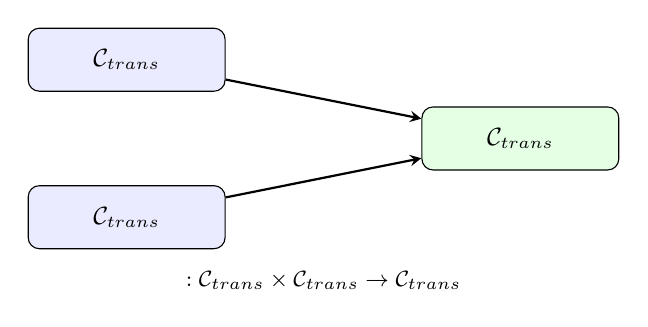
\begin{tikzpicture}[font=\small, arr/.style={->, thick, >=stealth}]
  % 双函子
  \node[draw, rounded corners, fill=blue!8, minimum width=2.5cm, minimum height=0.8cm] (A) at (0,1) {$\mathcal C_{\text{trans}}$};
  \node[draw, rounded corners, fill=blue!8, minimum width=2.5cm, minimum height=0.8cm] (B) at (0,-1) {$\mathcal C_{\text{trans}}$};
  \node[draw, rounded corners, fill=green!10, minimum width=2.5cm, minimum height=0.8cm] (C) at (5,0) {$\mathcal C_{\text{trans}}$};
  \draw[arr] (A) -- node[above, font=\footnotesize]{$\circledast$} (C);
  \draw[arr] (B) -- (C);
  \node[font=\footnotesize] at (2.5,-1.8) {$\circledast:\mathcal C_{\text{trans}}\times\mathcal C_{\text{trans}}\to\mathcal C_{\text{trans}}$};
\end{tikzpicture}
\caption{周期卷积双函子：双变量输入，保留全部频率对交互。}
\label{fig:periodic_convolution_bifunctor}
\end{figure}

\section{周期流形的范畴论表述}\label{sec:periodic_manifold_category}

\begin{definition}[离散格点范畴]\label{def:discrete_lattice_category}
设 $\mathcal{L}$ 为离散时空格点（“周期流形”章定义 \ref{def:discrete_spacetime_lattice}）。\textbf{离散格点范畴} $\mathbf{Latt}$ 定义为：
\begin{enumerate}[label=(\roman*)]
    \item \textbf{对象}：格点上的势矢量场 $\mathbf{V}: \mathcal{L} \to \mathbb{R}^d$（或 $\mathbb{C}^d$）。
    \item \textbf{态射}：格点间的离散平移 $\mathcal{T}_{\mathbf{m}}$、离散旋转 $\mathcal{R}_\theta$、离散缩放 $\mathcal{S}_\alpha$，以及它们的复合。
\end{enumerate}
\end{definition}

\begin{definition}[连续极限函子]\label{def:continuum_limit_functor}
\textbf{连续极限函子} $\mathcal{C}_{\infty}: \mathbf{Latt} \to \mathbf{Man}$ 将离散格点流形映射为其连续极限：
\[
\mathcal{C}_{\infty}(\mathcal{L}) = \lim_{\Delta x \to 0} \mathcal{L}_{\Delta x}.
\]
\end{definition}

\begin{proposition}[连续极限函子与伴随性]\label{prop:continuum_limit_adjunction}
连续极限函子 $\mathcal{C}_{\infty}$ 与离散化函子 $\mathcal{D}: \mathbf{Man} \to \mathbf{Latt}$ 构成一对伴随：
\[
\mathcal{D} \dashv \mathcal{C}_{\infty}.
\]
\end{proposition}

\begin{proof}
构造伴随的自然双射（定义 \ref{def:adjoint_functor}）：
\[
\operatorname{Hom}_{\mathbf{Latt}}(\mathcal{D}M, L) \cong \operatorname{Hom}_{\mathbf{Man}}(M, \mathcal{C}_{\infty}L).
\]
从右到左：连续映射 $\varphi: M \to \mathcal{C}_{\infty}L$ 在离散化格点上的限制给出格点态射。从左到右：格点态射嵌入极限后由连续极限的唯一确定性（“周期流形”章定理 \ref{thm:continuum_limit_full}）唯一延拓为连续映射。两映射互逆，故 $\mathcal{D} \dashv \mathcal{C}_{\infty}$。
\end{proof}

\begin{remark}[与“周期流形”章的接口]\label{ch13_periodic_manifold_interface_remark}
离散格点范畴 $\mathbf{Latt}$ 的态射族 $\{\mathcal{T}_{\mathbf{m}}, \mathcal{R}_\theta, \mathcal{S}_\alpha\}$ 对应“周期流形”章三种基本操作，连续极限函子 $\mathcal{C}_{\infty}$ 是该章连续极限定理（定理 \ref{thm:continuum_limit_full}）的函子化。离散曲率与 Wilson 环对应 $\mathbf{Latt}$ 中的闭环态射。
\end{remark}

\section{置闰函子：不可公度周期的范畴修正}\label{sec:intercalation_functor}

\begin{remark}[本节定位]\label{rem:intercalation_functor_positioning}
前节“周期流形的范畴论表述”建立了连续极限函子 $\mathcal{C}_\infty:\mathbf{Latt}\to\mathbf{Man}$ 及其左伴随——离散化函子 $\mathcal{D}:\mathbf{Man}\to\mathbf{Latt}$。然而，当连续周期 $T_F$ 与采样步长 $\Delta x$ 不可公度（即理想周期比 $\rho = T_F/\Delta x \notin \mathbb{Q}$）时，均匀采样序列不再具有严格整数周期，离散化函子 $\mathcal{D}$ 在此情形下不保持周期结构——这是范畴链条上的一处逻辑缺口。

本节引入\textbf{置闰函子} $\mathcal{R}:\mathcal{C}_{\text{cont}}\to\mathcal{C}_{\text{trans}}$ 修复这一缺口。其核心思想为：用整数列 $\{N_m\}$ 逼近理想周期比 $\rho$，使累计采样误差有界。置闰函子在范畴层面携带三项结构——\textbf{置闰对象}（定义 \ref{def:intercalation_object}）、\textbf{置闰序列的函子性}（定理 \ref{thm:intercalation_functoriality}）与\textbf{与连续极限函子的交换律}（定理 \ref{thm:intercalation_continuum_commutation}）。

本节七主题定位：平移——置闰序列的累计采样数 $S_M$ 逼近 $M\rho$ 的平移累积（定义 \ref{def:intercalation_object}）；缩放——理想周期比 $\rho$ 作为标度荷（定义 \ref{def:ideal_period_ratio_categorical}）；旋转——置闰误差的相位修正（定理 \ref{thm:intercalation_phase_correction}）；守恒——累计误差有界性（引理 \ref{lem:intercalation_error_bound_category}）；对称——连分数收敛子的对称逼近（定理 \ref{thm:intercalation_continued_fraction}）；闭合——置闰窗口使近似周期闭合（推论 \ref{cor:intercalation_window_closure}）；周期——$\rho \in \mathbb{Q}$ 时退化为严格周期函子（命题 \ref{prop:intercalation_rational_degeneracy}）。
\end{remark}

\subsection{公度性缺口与置闰对象}

\begin{definition}[范畴层面的理想周期比]\label{def:ideal_period_ratio_categorical}
设 $\mathcal{C}_{\text{cont}}$ 为连续周期范畴——对象为连续 $T_F$-周期函数 $F:\mathbb{R}\to\mathbb{C}$，态射为与时间平移交换的线性映射。设固定采样步长 $\Delta x > 0$。定义\textbf{范畴层面的理想周期比}为函子
\[
\rho:\mathcal{C}_{\text{cont}}\to\mathbb{R}_{>0},\qquad
\rho(F)=\frac{T_F}{\Delta x}.
\]
称 $\rho(F)$ 为对象 $F$ 的\textbf{标度荷}。$F$ 在 $\Delta x$ 下\textbf{公度}，若 $\rho(F)\in\mathbb{Q}$；否则称 $F$ 在 $\Delta x$ 下\textbf{非公度}。
\end{definition}

\begin{proposition}[公度性缺口]\label{prop:commensurability_gap}
设 $F$ 为连续 $T_F$-周期函数，$\Delta x>0$，$\rho = T_F/\Delta x$。
\begin{enumerate}[label=(\roman*)]
    \item 若 $\rho\in\mathbb{N}^+$，则均匀采样序列 $f(n)=F(n\Delta x)$ 是 $T=\rho$ 的离散周期函数，离散化函子 $\mathcal{D}$ 在 $F$ 上保持周期结构；
    \item 若 $\rho\in\mathbb{Q}\setminus\mathbb{N}^+$，$\rho=p/q$（既约），则 $f$ 是 $T=p$ 的离散周期函数，$\mathcal{D}$ 仍保持周期结构；
    \item 若 $\rho\notin\mathbb{Q}$，则 $f$ 不具有任何非零周期，$\mathcal{D}$ 在 $F$ 上不保持周期结构——范畴链条在 $\mathcal{D}$ 处断裂。
\end{enumerate}
\end{proposition}

\begin{proof}
(i)(ii) 由“离散采样逼近与置闰”章命题 \ref{prop:commensurability_periodicity_parallel} 直接得出。(iii) 假设 $f$ 具有非零周期 $T\in\mathbb{N}^+$，则 $F(T\Delta x)=F(0)$，由 $F$ 以 $T_F$ 为基本周期存在整数 $m$ 使 $T\Delta x=mT_F$，即 $\rho=T/m\in\mathbb{Q}$，与 $\rho\notin\mathbb{Q}$ 矛盾。故 $\operatorname{Group}_{\mathrm{period}}(f)=\{0\}$。
\end{proof}

\begin{definition}[置闰对象]\label{def:intercalation_object}
设 $F\in\mathcal{C}_{\text{cont}}$ 非公度，$\rho=\rho(F)\in\mathbb{R}_{>0}\setminus\mathbb{Q}$。$F$ 的一个\textbf{置闰对象}是一个四元组
\[
(F,\;\{N_m\}_{m\in\mathbb{N}},\;\{S_M\}_{M\in\mathbb{N}},\;E),
\]
其中：
\begin{enumerate}[label=(\roman*)]
    \item $\{N_m\}$ 为 $\rho$ 的置闰序列：$N_m\in\{\lfloor\rho\rfloor,\lceil\rho\rceil\}$ 且 $\lim_{M\to\infty}\frac{1}{M}\sum_{m=0}^{M-1}N_m=\rho$；
    \item $S_M=\sum_{m=0}^{M-1}N_m$ 为累计采样数；
    \item $E:\mathbb{N}\to\mathbb{R}$，$E(M)=S_M-M\rho$ 为置闰误差，且存在常数 $C>0$ 使 $|E(M)|\le C$ 对一切 $M$ 成立。
\end{enumerate}
记 $\mathbf{Int}(\rho)$ 为 $\rho$ 上全体置闰对象构成的类。
\end{definition}

\begin{remark}[置闰对象与观测窗口]\label{rem:intercalation_object_window}
置闰对象 $(F,\{N_m\},\{S_M\},E)$ 的核心几何含义是：以 $S_M$ 为窗口长度截取连续对象 $F$ 的采样序列，所得的 $S_M$ 长离散序列在窗口内近似包含 $M$ 个连续周期。窗口 $[0,S_M]$ 称为\textbf{置闰窗口}。由误差有界性，$S_M-M\rho$ 不随 $M$ 增长——累计相位误差被约束在有界带内。
\end{remark}

\begin{lemma}[置闰误差有界性]\label{lem:intercalation_error_bound_category}
设 $\rho>0$，$\{N_m\}$ 为 $\rho$ 的基本置闰序列（下、上、平衡三种之一），$S_M=\sum_{m=0}^{M-1}N_m$，$E(M)=S_M-M\rho$。则
\[
|E(M)|\le \tfrac{1}{2}
\]
对平衡置闰成立，对下置闰 $E(M)\in(-1,0]$，对上置闰 $E(M)\in[0,1)$。特别地，三种基本置闰序列均给出置闰对象（取 $C=1$）。
\end{lemma}

\begin{proof}
由“离散采样逼近与置闰”章定理 \ref{thm:intercalation_error_bound_parallel} 直接给出。
\end{proof}

\begin{figure}[htbp]
\centering
\begin{tikzpicture}[scale=0.9]
  % 理想采样位置
  \draw[->, thick, >=stealth] (0,0) -- (10,0);
  \foreach \x in {0,2.5,5,7.5,10} {
    \draw[gray, dashed] (\x,0) -- (\x,-1.5);
  }
  \node[font=\footnotesize] at (0,-1.8) {$0$};
  \node[font=\footnotesize] at (2.5,-1.8) {$\rho$};
  \node[font=\footnotesize] at (5,-1.8) {$2\rho$};
  \node[font=\footnotesize] at (7.5,-1.8) {$3\rho$};
  % 实际采样位置（整数）
  \foreach \x in {0,3,5,8,10} {
    \draw[thick, red] (\x,0.3) -- (\x,-0.3);
    \node[circle, fill, red, inner sep=1.5pt] at (\x,0) {};
  }
  \node[red, font=\footnotesize] at (3,0.6) {$N_0=3$};
  \node[red, font=\footnotesize] at (5,0.6) {$N_1=2$};
  \node[red, font=\footnotesize] at (8,0.6) {$N_2=3$};
  % 误差
  \draw[<->, thick, orange, >=stealth] (5,0.3) -- (7.5,0.3);
  \node[orange, font=\footnotesize] at (6.3,0.6) {$E$};
  \node at (5,-2.5) {置闰窗口 $[0,S_M]$：累计误差有界};
\end{tikzpicture}
\caption{置闰序列：理想采样位置（虚线）与实际整数采样位置（红点）的偏差被约束在有界带内。}
\label{fig:intercalation_error}
\end{figure}

\subsection{置闰函子}

\begin{definition}[置闰函子]\label{def:intercalation_functor}
设固定采样步长 $\Delta x>0$ 与置闰模式（下/上/平衡）。定义\textbf{置闰函子}
\[
\mathcal{R}:\mathcal{C}_{\text{cont}}\to\mathcal{C}_{\text{trans}}
\]
为：
\begin{enumerate}[label=(\roman*)]
    \item \textbf{对象层面}：对 $F\in\mathcal{C}_{\text{cont}}$，置 $\rho=\rho(F)$。若 $\rho\in\mathbb{Q}$，令 $\mathcal{R}(F)$ 为 $\mathcal{D}(F)$ 的任意严格周期延拓（在 $\mathcal{C}_{\text{trans}}$ 中良定义）。若 $\rho\notin\mathbb{Q}$，令
    \[
    \mathcal{R}(F)(n)=F(n\Delta x),\qquad n=0,1,\dots,S_M-1,\quad M\ \text{随窗口确定},
    \]
    并在 $\mathcal{C}_{\text{trans}}$ 中取其在置闰窗口上的 $S_M$-周期延拓。
    \item \textbf{态射层面}：对 $\mathcal{C}_{\text{cont}}$ 中态射 $h:F\to G$（与时间平移交换的线性映射），定义 $\mathcal{R}(h)$ 为限制在置闰窗口上的 $S_M$-周期序列之间的线性映射。
\end{enumerate}
\end{definition}

\begin{theorem}[置闰函子的函子性]\label{thm:intercalation_functoriality}
置闰函子 $\mathcal{R}$ 保持恒等态射与复合：
\begin{enumerate}[label=(\roman*)]
    \item $\mathcal{R}(\operatorname{id}_F)=\operatorname{id}_{\mathcal{R}(F)}$；
    \item 对 $\mathcal{C}_{\text{cont}}$ 中的复合 $h_2\circ h_1$，有 $\mathcal{R}(h_2\circ h_1)=\mathcal{R}(h_2)\circ\mathcal{R}(h_1)$。
\end{enumerate}
\end{theorem}

\begin{proof}
(i) $\operatorname{id}_F$ 在采样点 $n\Delta x$ 处的限制为恒等映射，置闰延拓后仍为恒等序列。

(ii) 设 $h_1:F\to G$，$h_2:G\to K$ 为 $\mathcal{C}_{\text{cont}}$ 中的态射。对任意采样点 $n\Delta x$（$n\in[0,S_M)$），
\[
[\mathcal{R}(h_2\circ h_1)](n)=(h_2\circ h_1)(F)(n\Delta x)=h_2(h_1(F(n\Delta x)))=[\mathcal{R}(h_2)\circ\mathcal{R}(h_1)](n).
\]
在置闰窗口上的逐点等式延拓为 $S_M$-周期序列的等式，故 $\mathcal{R}$ 保持复合。
\end{proof}

\begin{proposition}[公度情形的退化]\label{prop:intercalation_rational_degeneracy}
设 $F\in\mathcal{C}_{\text{cont}}$ 在 $\Delta x$ 下公度，即 $\rho(F)=p/q\in\mathbb{Q}$（既约）。则置闰函子退化为离散化函子：$\mathcal{R}(F)\cong\mathcal{D}(F)$，且 $\operatorname{Group}_{\mathrm{period}}(\mathcal{R}(F))=p\mathbb{Z}$。特别地，置闰序列为常数列 $N_m\equiv p$，置闰误差恒为零。
\end{proposition}

\begin{proof}
由命题 \ref{prop:commensurability_gap}(ii)，$f(n)=F(n\Delta x)$ 以 $p$ 为周期。置闰序列取常数列 $N_m=p$ 时，$S_M=Mp$，故 $E(M)=Mp-Mp=0$。置闰窗口延拓与 $\mathcal{D}(F)$ 的严格 $p$-周期延拓一致。故 $\mathcal{R}(F)\cong\mathcal{D}(F)$ 且 $\operatorname{Group}_{\mathrm{period}}(\mathcal{R}(F))=p\mathbb{Z}$。
\end{proof}

\begin{theorem}[置闰函子的相位修正]\label{thm:intercalation_phase_correction}
设 $F\in\mathcal{C}_{\text{cont}}$ 非公度，$\rho=\rho(F)\notin\mathbb{Q}$，$\{N_m\}$ 为 $\rho$ 的平衡置闰序列。则对置闰窗口 $[0,S_M]$ 上的连续傅里叶级数 $\displaystyle F(t)=\sum_{m\in\mathbb{Z}}c_m e^{i2\pi mt/T_F}$，采样序列 $f(n)=F(n\Delta x)$ 的 $S_M$ 点 DFT 满足
\[
\hat{f}(k)=\sum_{m\in\mathbb{Z}}c_m\,D_{S_M}\!\left(\frac{m}{\rho}-\frac{k}{S_M}\right),
\]
其中 $D_T(\theta)=\dfrac{1}{T}\sum_{n=0}^{T-1}e^{i2\pi n\theta}$ 为 Dirichlet 核，且主瓣偏移满足
\[
\left|\frac{m}{\rho}-\frac{k}{S_M}\right|\le\frac{|m|\,|E(M)|}{\rho\,S_M}\le\frac{|m|}{2\rho S_M}.
\]
即置闰函子在频域上把非公度连续对象映射为\textbf{有界相位误差}的离散对象——相位误差由置闰误差 $E(M)$ 控制。
\end{theorem}

\begin{proof}
由“调和分析”章定理 \ref{thm:intercalation_dft_leakage}（置闰窗口的 DFT 泄漏估计）直接得到，其中平衡置闰给出 $|E(M)|\le 1/2$。
\end{proof}

\begin{corollary}[置闰窗口的相位闭合]\label{cor:intercalation_window_closure}
设 $\rho\notin\mathbb{Q}$，$\{p_j/q_j\}$ 为 $\rho$ 的连分数收敛子。取 $T=p_j$，$M=q_j$（置闰窗口为 $[0,p_j]$）。则置闰窗口内的累计误差
\[
|E(q_j)|=|p_j-q_j\rho|<\frac{1}{q_{j+1}},
\]
且窗口内近似闭合 $M=q_j$ 个连续周期——置闰函子 $\mathcal{R}(F)$ 在窗口 $[0,p_j]$ 上以 $S_M=p_j$ 为周期延拓时，相位误差小于 $1/q_{j+1}$。
\end{corollary}

\begin{proof}
由“离散采样逼近与置闰”章定理 \ref{thm:continued_fraction_best_approx_parallel} 与定理 \ref{thm:intercalation_phase_correction} 直接得出。
\end{proof}

\begin{theorem}[连分数最佳置闰函子的普适性]\label{thm:intercalation_continued_fraction}
设 $\rho>0$ 无理，$\{p_j/q_j\}$ 为其连分数收敛子。则置闰函子 $\mathcal{R}$ 在上述窗口序列 $\{(p_j,q_j)\}_{j\ge 0}$ 上满足
\[
\lim_{j\to\infty}\frac{|E(q_j)|}{p_j}=0,\qquad
\frac{|E(q_j)|}{p_j}<\frac{1}{p_j q_{j+1}}\to 0.
\]
即在连分数收敛窗口序列上，置闰函子 $\mathcal{R}$ 的\textbf{相对相位误差}趋于零——置闰函子在极限意义下\textbf{恢复了} $\mathcal{C}_{\text{cont}}$ 与 $\mathcal{C}_{\text{trans}}$ 之间被公度性缺口切断的范畴联系。
\end{theorem}

\begin{proof}
由定理 \ref{thm:intercalation_phase_correction} 的主瓣偏移界 $|m|\,|E|/(\rho S_M)$ 与推论 \ref{cor:intercalation_window_closure} 的 $|E(q_j)|<1/q_{j+1}$，得
\[
\frac{|E(q_j)|}{p_j}<\frac{1}{p_j q_{j+1}}.
\]
由连分数理论 $p_j,q_j\to\infty$ 且 $q_{j+1}>q_j$，故 $1/(p_j q_{j+1})\to 0$。
\end{proof}

\subsection{置闰函子与连续极限函子的交换}

\begin{theorem}[置闰函子与连续极限函子的交换律]\label{thm:intercalation_continuum_commutation}
设 $\mathcal{D}:\mathbf{Man}\to\mathbf{Latt}$ 为离散化函子，$\mathcal{C}_\infty:\mathbf{Latt}\to\mathbf{Man}$ 为连续极限函子（前节定义 \ref{def:continuum_limit_functor}），$\mathcal{R}:\mathcal{C}_{\text{cont}}\to\mathcal{C}_{\text{trans}}$ 为置闰函子。则以下图表在极限意义下交换：
\[
\begin{tikzcd}[row sep=large, column sep=large]
\mathcal{C}_{\text{cont}} \arrow[r, "\mathcal{R}"] \arrow[d, "\text{嵌入}"'] & \mathcal{C}_{\text{trans}} \arrow[d, "\mathcal{D}"] \\
\mathbf{Man} \arrow[r, "\mathcal{C}_\infty"'] & \mathbf{Latt}
\end{tikzcd}
\]
更精确地：对 $F\in\mathcal{C}_{\text{cont}}$，取置闰窗口序列 $\{(p_j,q_j)\}_{j\ge 0}$（$p_j\to\infty$），则
\[
\lim_{j\to\infty}\mathcal{D}\big(\mathcal{R}_j(F)\big)=\mathcal{D}\big(\mathcal{D}(F)\big),
\]
其中 $\mathcal{R}_j$ 表示在第 $j$ 个置闰窗口上的置闰函子，$\mathcal{D}(\mathcal{R}_j(F))$ 为置闰序列在格点上的实现。
\end{theorem}

\begin{proof}
由定理 \ref{thm:intercalation_continued_fraction}，在第 $j$ 个窗口上，置闰序列 $\mathcal{R}_j(F)$ 的相对相位误差趋于零。故在窗口 $[0,p_j]$ 上，$\mathcal{R}_j(F)$ 与 $\mathcal{D}(F)$ 的差在有界误差意义下趋于零。取 $j\to\infty$，两离散序列在格点范畴中收敛到同一对象。
\end{proof}

\begin{remark}[置闰函子的范畴论地位]\label{rem:intercalation_category_status}
置闰函子 $\mathcal{R}$ 与离散化函子 $\mathcal{D}$ 的关系可理解为：$\mathcal{R}$ 是 $\mathcal{D}$ 在非公度情形下的\textbf{有界误差修正}。当 $\rho\in\mathbb{Q}$ 时二者同构（命题 \ref{prop:intercalation_rational_degeneracy}）；当 $\rho\notin\mathbb{Q}$ 时，$\mathcal{R}$ 通过选择连分数收敛窗口使相位误差趋于零（定理 \ref{thm:intercalation_continued_fraction}），从而在极限意义下恢复 $\mathcal{D}$ 的范畴性。

从伴随函子的视角看，若将离散化函子 $\mathcal{D}$ 视为左伴随、连续极限函子 $\mathcal{C}_\infty$ 视为右伴随（前节命题 \ref{prop:continuum_limit_adjunction}），则置闰函子 $\mathcal{R}$ 可视为伴随对 $(\mathcal{D},\mathcal{C}_\infty)$ 在非公度情形下的\textbf{一致性修正}——它不改变伴随对本身，而是在对象层面携带修正数据，使伴随的自然同构在非公度情形下保持到任意精度。
\end{remark}

\begin{proposition}[置闰函子的守恒量]\label{prop:intercalation_conservation}
置闰函子 $\mathcal{R}$ 在对象层面携带以下守恒量：
\begin{enumerate}[label=(\roman*)]
    \item \textbf{累计误差有界性}：$|E(M)|\le C$ 对一切 $M$ 成立——置闰序列的相位误差在窗口尺度上守恒有界；
    \item \textbf{相对误差单调收敛}：$\displaystyle\lim_{j\to\infty}\frac{|E(q_j)|}{p_j}=0$——连分数收敛窗口上的相对相位误差趋于零；
    \item \textbf{能量守恒}：置闰窗口上的 DFT 帕塞瓦尔恒等式
    \[
    \sum_{n=0}^{S_M-1}|f(n)|^2=S_M\sum_{k=0}^{S_M-1}|\hat{f}(k)|^2
    \]
    在置闰窗口上精确成立——置闰不改变窗口内的总能量。
\end{enumerate}
\end{proposition}

\begin{proof}
(i) 由引理 \ref{lem:intercalation_error_bound_category}。(ii) 由定理 \ref{thm:intercalation_continued_fraction}。(iii) 由“离散采样逼近与置闰”章定理 \ref{thm:discrete_parseval_parallel} 在置闰窗口上的应用。
\end{proof}

\begin{remark}[置闰函子与观察者函子的接口]\label{rem:intercalation_observer_interface}
置闰函子 $\mathcal{R}$ 与观察者函子 $\mathcal{P}$（下节定义 \ref{def:observer_functor}）的关系为：观察者函子提取可观测痕迹，而置闰函子确定观察者采样窗口的最优长度。具体地，置闰函子给出窗口序列 $\{(p_j,q_j)\}$，观察者函子在该窗口上投影出可观测痕迹——置闰使观察者采样窗口近似包含整数个连续周期，从而使投影的相位误差最小化。二者合起来构成“采样—投影”双重函子
\[
\mathcal{C}_{\text{cont}}\xrightarrow{\mathcal{R}}\mathcal{C}_{\text{trans}}\xrightarrow{\mathcal{P}}\mathcal{C}_{\text{obs}},
\]
其中 $\mathcal{R}$ 使相位误差有界，$\mathcal{P}$ 使结构投影保形。
\end{remark}

\begin{figure}[htbp]
\centering
\begin{tikzcd}[row sep=large, column sep=large]
\mathcal{C}_{\text{cont}} \arrow[r, "\mathcal{R}"] \arrow[d, "\text{嵌入}"'] & \mathcal{C}_{\text{trans}} \arrow[d, "\mathcal{D}"] \\
\mathbf{Man} \arrow[r, "\mathcal{C}_\infty"'] & \mathbf{Latt}
\end{tikzcd}
\caption{置闰函子与连续极限函子的交换图：在极限意义下交换。}
\label{fig:intercalation_commutation}
\end{figure}

\section{观察者作为函子}\label{sec:observer_functor}

\begin{definition}[观察者函子]\label{def:observer_functor}
\textbf{观察者函子} $\mathcal{P}: \mathcal{C}_{\text{trans}} \times \mathcal{C}_{\text{rot}} \to \mathcal{C}_{\text{obs}}$ 将时间周期范畴和旋转周期范畴的乘积映射到\textbf{可观测痕迹范畴} $\mathcal{C}_{\text{obs}}$：
\[
\mathcal{P}(f_T, f_S) = \mathcal{N}(r, \sigma) \cdot \left( \Phi(f_T) \cdot \nabla S + \Phi(f_S) \cdot \nabla S \right) \cdot \mathbf{u}_P,
\]
其中 $\mathcal{N}(r, \sigma) = (\sigma/(r^2+\sigma))^2$ 为采样归一化因子，$\Phi$ 为相位提取函子，$\mathbf{u}_P$ 为观察者视线方向。
\end{definition}

\begin{theorem}[观察者函子的分解]\label{thm:observer_functor_decomposition}
观察者函子 $\mathcal{P}$ 可分解为三个子函子的复合：
\[
\mathcal{P} = \mathcal{P}_{\cdot} \circ \operatorname{add} \circ (\mathcal{P}_{\nabla} \times \mathcal{P}_{\times}),
\]
其中 $\mathcal{P}_{\nabla}$ 将时间通量投影为可观测场的无旋部分，$\mathcal{P}_{\times}$ 将空间通量投影为无散部分，$\mathcal{P}_{\cdot}$ 施加归一化因子。
\end{theorem}

\begin{proof}
由定义 \ref{def:observer_functor} 的显式公式逐项分解。无旋/无散的分解由“矢量分析”章亥姆霍兹分解定理（定理 \ref{thm:helmholtz}）保证。
\end{proof}

\begin{corollary}[观察者函子与伴随性]\label{cor:observer_adjunction}
观察者函子 $\mathcal{P}$ 存在左伴随 $\mathcal{P}^*$（重构函子），构成一对伴随：
\[
\mathcal{P}^* \dashv \mathcal{P}.
\]
伴随的单位 $\eta$ 不是同构——观察过程中的信息丢失是不可逆的。
\end{corollary}

\begin{proof}
构造 $\mathcal{P}^*$ 为典型提升：对每个痕迹 $O$，取 $\mathcal{P}^*(O)$ 为满足 $\mathcal{P}(\mathcal{P}^*(O)) = O$ 的极小范数原像。伴随双射由线性结构给出。单位 $\eta$ 不是同构因为典型提升不是观察的截面。
\end{proof}

\begin{remark}[观察者函子与守恒律破缺]\label{rem:observer_conservation_breaking}
伴随的单位 $\eta$ 不是同构，意味着观察者无法从可观测痕迹中完全重构原始的周期结构。观察过程中的信息丢失是不可逆的——时间系统和空间系统的守恒量（能量、角动量）被观察系统的散度（对称中心 $1$）（采样衰减、投影选择）部分破坏。
\end{remark}

\begin{figure}[htbp]
\centering
\begin{tikzpicture}[font=\small, arr/.style={->, thick, >=stealth}]
  \node[draw, rounded corners, fill=blue!8, minimum width=2.5cm, minimum height=0.8cm] (T) at (0,1) {$\mathcal C_{\text{trans}}$};
  \node[draw, rounded corners, fill=red!8, minimum width=2.5cm, minimum height=0.8cm] (R) at (0,-1) {$\mathcal C_{\text{rot}}$};
  \node[draw, rounded corners, fill=green!10, minimum width=2.5cm, minimum height=0.8cm] (O) at (5,0) {$\mathcal C_{\text{obs}}$};
  \draw[arr] (T) -- node[above, font=\footnotesize]{$\mathcal P$} (O);
  \draw[arr] (R) -- (O);
  \node[font=\footnotesize] at (2.5,-1.8) {观察者函子：时间+空间 $\to$ 可观测痕迹};
\end{tikzpicture}
\caption{观察者函子 $\mathcal{P}$：将时间周期范畴与旋转周期范畴的乘积投影为可观测痕迹范畴。}
\label{fig:observer_functor}
\end{figure}

\section{周期范畴与守恒律}\label{sec:periodic_category_conservation_laws}

\begin{theorem}[诺特定理的范畴论表述]\label{thm:noether_categorical}
设 $\mathcal{C}^G$ 为 $G$-周期范畴，其中 $G$ 为李群。存在一个自然同构：
\[
\operatorname{Symmetry}(\mathcal{C}^G) \cong \operatorname{Conserved}(\mathcal{C}^G),
\]
其中 $\operatorname{Symmetry}(\mathcal{C}^G)$ 是 $\mathcal{C}^G$ 的连续对称性群，$\operatorname{Conserved}(\mathcal{C}^G)$ 是 $\mathcal{C}^G$ 的守恒量空间。

具体而言：
\begin{enumerate}[label=(\roman*)]
    \item 平移对称性（$G = \mathbb{R}$，$0$-对称）$\cong$ 能量/动量守恒。
    \item 旋转对称性（$G = U(1)$，$i$-对称）$\cong$ 角动量守恒。
    \item 缩放对称性（$G = \mathbb{R}^+$，$1$-对称）$\cong$ 标度荷守恒。
\end{enumerate}
\end{theorem}

\begin{proof}
对每个对象 $(X, \rho) \in \mathcal{C}^G$：$G$ 的每个单参数子群经作用 $\rho$ 给出 $X$ 上的单参数自同构族，其无穷小生成元对应的诺特荷即守恒量（“周期函数与具有周期轨道的群”章定理 \ref{thm:noether_group_with_periodic_orbits}）。自然性由周期态射的等变性给出。
\end{proof}

\begin{figure}[htbp]
\centering
\begin{tikzpicture}[font=\small, arr/.style={->, thick, >=stealth}]
  \node[draw, rounded corners, fill=blue!8, minimum width=3cm, minimum height=0.8cm, align=center] (sym) {对称性群\\$\operatorname{Symmetry}$};
  \node[draw, rounded corners, fill=green!10, minimum width=3cm, minimum height=0.8cm, align=center] (cons) at (6,0) {守恒量空间\\$\operatorname{Conserved}$};
  \draw[<->, thick, >=stealth] (sym) -- node[above, font=\footnotesize]{自然同构} node[below, font=\footnotesize]{Noether} (cons);
  \node[font=\footnotesize] at (3,-1.2) {$\operatorname{Symmetry}(\mathcal C^G)\cong\operatorname{Conserved}(\mathcal C^G)$};
\end{tikzpicture}
\caption{诺特定理的范畴论表述：对称性群与守恒量空间的自然同构。}
\label{fig:noether_categorical}
\end{figure}

\section{周期范畴的统一视角}\label{sec:periodic_category_unification}

\begin{theorem}[周期数学的范畴论统一]\label{thm:periodic_category_unification}
周期数学的核心结构可以通过以下交换图统一表述：
\[
\begin{tikzcd}
\mathcal{C}_{\text{scal}} \arrow[r, "\mathcal{L}"] \arrow[d, "\mathcal{F}_{\text{scal}}"'] & \mathcal{C}_{\text{trans}} \arrow[d, "\mathcal{F}_{\text{trans}}"] \\
\mathbf{Vect}_{\mathbb{C}} \arrow[r, "\mathcal{L}_*"'] & \mathbf{Vect}_{\mathbb{C}}
\end{tikzcd}
\]
其中 $\mathcal{L}$ 为对数函子，$\mathcal{F}_{\text{trans}}$ 为傅里叶变换，$\mathcal{F}_{\text{scal}}$ 为梅林变换。左方块的交换性由换元 $x = e^t$ 直接验证。
\end{theorem}

\begin{proof}
由换元 $x = e^t$，缩放周期函数 $f(x)$ 变为平移周期函数 $g(t) = f(e^t)$。梅林变换 $\mathcal{F}_{\text{scal}}$ 与傅里叶变换 $\mathcal{F}_{\text{trans}}$ 在该换元下交换：$\mathcal{F}_{\text{trans}}(\mathcal{L}f) = \mathcal{L}_*(\mathcal{F}_{\text{scal}}f)$。守恒结构由定理 \ref{thm:noether_categorical} 和帕塞瓦尔恒等式保证。
\end{proof}

\begin{remark}[周期范畴在全书中的枢纽地位]\label{rem:periodic_category_hub}
周期范畴是周期数学理论体系的最高抽象层。它将“周期基础”章的群表示论原型、“数系”章的对称中心、“标量与矢量”章的相似度与趋势、“函数与极限”章的微积分基础、“级数与卷积”章的周期变换与卷积、“周期流形”章的离散几何——全部统一纳入范畴论的语言。

在这个统一的框架中：
\begin{itemize}
    \item \textbf{周期}是群作用下的不变性在范畴论层面的自然表达——$G$-周期对象 $(X, \rho)$。
    \item \textbf{守恒律}是连续对称性的诺特荷在函子层面的自然同构——\\$\operatorname{Symmetry} \cong \operatorname{Conserved}$。
    \item \textbf{相位}是范畴上的结构保持映射——所有周期的任意相位都可以作为函子（推论 \ref{cor:all_phases_functorial}）。
    \item \textbf{微分与积分}是周期范畴上的伴随算子对——$\mathcal{D} \dashv \mathcal{I}$。
    \item \textbf{卷积与周期卷积}是周期范畴上的双函子——$*$ 和 $\circledast$。
    \item \textbf{观察者}是连接时间系统和空间系统的核心函子——$\mathcal{P}$。
\end{itemize}
\end{remark}

\begin{remark}[高阶范畴展望]\label{ch13_higher_category_remark}
本章把自然变换（定义 \ref{def:natural_transformation}）作为最高层级结构。一个自然的下一步是把自然变换之间的态射——修改（modification）——纳入框架：周期参数族的连续变化正是修改的实例，此时周期范畴组织为一个 $2$-范畴。观察者函子的伴随单位不是同构说明观测-重构循环在 $2$-范畴层面形成一个不可逆的 $2$-态射。此为展望性注释，不立定理。
\end{remark}

\section*{本章七主题对照表}

\begin{figure}[htbp]
\centering
\begin{tikzpicture}[
  theme/.style={draw, rounded corners, fill=green!10, minimum width=1.2cm, minimum height=0.55cm, align=center, font=\footnotesize}
]
  \node[theme] (p) at (0,0) {平移};
  \node[theme, right=0.3cm of p] (s) {缩放};
  \node[theme, right=0.3cm of s] (r) {旋转};
  \node[theme, right=0.3cm of r] (c) {守恒};
  \node[theme, right=0.3cm of c] (sym) {对称};
  \node[theme, right=0.3cm of sym] (cl) {闭合};
  \node[theme, right=0.3cm of cl] (per) {周期};
  \node[draw, dashed, rounded corners, fit=(p)(per), inner sep=6pt] (box) {};
  \node[below=0.1cm of box, font=\footnotesize] {七大主题贯穿周期范畴};
\end{tikzpicture}
\caption{本章七大主题：平移、缩放、旋转、守恒、对称、闭合、周期。}
\label{fig:periodic_category_themes}
\end{figure}

\begin{center}
\begin{tabular}{>{\centering\arraybackslash}p{2.2cm}>{\centering\arraybackslash}p{10.5cm}}
\toprule
主题 & 本章对应 \\
\midrule
平移 & 平移周期范畴 $\mathcal{C}_{\text{trans}}$ 与微分算子 $\mathcal{D}$（$0$-对称）；置闰序列的累计采样数 $S_M$ 逼近 $M\rho$（定义 \ref{def:intercalation_object}） \\
缩放 & 缩放周期范畴与对数函子/指数函子（$1$-对称）；理想周期比 $\rho$ 作为标度荷（定义 \ref{def:ideal_period_ratio_categorical}） \\
旋转 & 旋转周期范畴、相位函子与傅里叶函子（$i$-对称）；置闰窗口的相位修正（定理 \ref{thm:intercalation_phase_correction}） \\
守恒 & 伴随算子的守恒条件（推论 \ref{cor:diff_int_conservation}）；诺特定理的范畴论表述（定理 \ref{thm:noether_categorical}）；置闰累计误差有界性（引理 \ref{lem:intercalation_error_bound_category}） \\
对称 & 自然同构与伴随对偶 $\mathcal{D}\dashv\mathcal{I}$；相位函子族 $\cong U(1)$（定理 \ref{thm:phase_functor_group}）；连分数收敛子的对称逼近（定理 \ref{thm:intercalation_continued_fraction}） \\
闭合 & 微分-积分算子的互逆闭合（引理 \ref{ch13_diff_int_inverse_lemma}）；周期卷积双函子的闭合格（定理 \ref{thm:periodic_convolution_functoriality}）；置闰窗口使近似周期闭合（推论 \ref{cor:intercalation_window_closure}） \\
周期 & 周期流形的范畴表述；相位函子的参数化（推论 \ref{cor:all_phases_functorial}）；$\rho\in\mathbb{Q}$ 时置闰函子退化为严格周期函子（命题 \ref{prop:intercalation_rational_degeneracy}） \\
\bottomrule
\end{tabular}
\end{center}

\section*{本章思考题}

\begin{enumerate}[leftmargin=3em, label=\textbf{题 \arabic*}]
    \item 根据定义 \ref{def:operator} 与定义 \ref{def:functor}，
    说明算子（自函子）与函子在作用域上的本质区别。
    请各举一例：一个算子保持周期类型不变，
    一个函子将平移周期范畴映射到另一个范畴（如傅里叶函子将周期函数映射为傅里叶系数序列）。

    \item 证明命题 \ref{prop:phase_functor_properties} 中相位函子
    $\Phi_{\theta,T}$ 的六条基本性质：
    函子性、保持周期、复合律、恒等元、逆元与幺正性。
    并验证定理 \ref{thm:phase_functor_group}：
    固定周期 $T$ 的相位函子族在复合下构成群，同构于 $U(1)$。

    \item 验证例 \ref{ex:phase_functor_action} 中相位函子对正弦函数的具体作用：
    取 $T=2\pi$，$f(t)=\sin t$，计算
    \[
    \Phi_{\pi/2,2\pi}(f)(t),\qquad
    \Phi_{\pi,2\pi}(f)(t).
    \]
    请说明为什么 $\Phi_{\pi,2\pi}$ 对正弦函数是恒等映射，
    并指出这与相位取 $\pi$ 时的对径关系有何联系。

    \item 证明引理 \ref{ch13_hom_frequency_lemma}：
    设 $f(t)=Ae^{i(\omega_1t+\varphi)}$，$g(t)=Be^{i(\omega_2t+\psi)}$ 为两个单周转圆对象。
    \begin{enumerate}[label=(\roman*)]
        \item 若 $\omega_1\neq\omega_2$，则 $\operatorname{Hom}(f,g)=\{0\}$；
        \item 若 $\omega_1=\omega_2=\omega$，则
              $\operatorname{Hom}(f,g)=\{c\cdot\frac{B}{A}e^{i(\psi-\varphi)}:c\in\mathbb{C}\}$。
    \end{enumerate}
    请说明为什么振幅与相位不是平移周期范畴的不变量
    （参见注 \ref{ch13_amplitude_phase_remark}）。

    \item 验证例 \ref{ch13_hom_set_example} 中三个单周转圆对象之间的态射计算：
    \[
    f(t)=3e^{i(2t+\pi/6)},\quad
    g(t)=2e^{i(3t-\pi/4)},\quad
    h(t)=5e^{i(2t+\pi/3)}.
    \]
    计算 $\operatorname{Hom}(f,g)$、$\operatorname{Hom}(f,h)$ 与 $\operatorname{Hom}(h,k)$（取 $k(t)=4e^{i2t}$），
    并验证复合律 $\mu\circ\lambda=\nu$。

    \item 证明定理 \ref{thm:diff_int_adjunction}：
    在平移周期范畴上，微分算子 $\mathcal{D}$ 与积分算子 $\mathcal{I}$
    构成伴随对 $\mathcal{D}\dashv\mathcal{I}$。
    请写出伴随的自然同构，并说明为什么需要零均值条件。

    \item 验证引理 \ref{ch13_diff_int_inverse_lemma}：
    \[
    (\mathcal{D}\circ\mathcal{I})(f)=f-\bar{f},\qquad
    (\mathcal{I}\circ\mathcal{D})(f)=f-f(0).
    \]
    在零均值周期函数的商范畴（模常数）上，二者互为严格逆。
    请用数值例子 \ref{ch13_adjunction_numeric_example} 验证。

    \item 证明命题 \ref{prop:three_category_functors}：
    三种周期范畴之间存在自然的函子——
    对数函子 $\mathcal{L}:\mathcal{C}_{\text{scal}}\to\mathcal{C}_{\text{trans}}$，
    指数函子 $\mathcal{E}:\mathcal{C}_{\text{trans}}\to\mathcal{C}_{\text{scal}}$，
    傅里叶函子 $\mathcal{F}:\mathcal{C}_{\text{trans}}\to\mathbf{Vect}_{\mathbb{C}}$。
    并证明推论 \ref{cor:grammar_adjunction}：$\mathcal{L}\dashv\mathcal{E}$。

    \item 证明定理 \ref{thm:periodic_convolution_functoriality_series}：
    周期卷积 $\circledast$ 是平移周期范畴上的双函子，满足
    保持恒等、保持复合、与相似度函子兼容、与趋势函子兼容。
    请说明周期卷积在频域中表现为张量积，相位与趋势在频域中表现为逐点运算。

    \item 证明命题 \ref{prop:commensurability_gap}：
    公度性缺口——当 $\rho=T_F/\Delta x\in\mathbb{Q}$ 时，
    离散化函子 $\mathcal{D}$ 保持周期结构；
    当 $\rho\notin\mathbb{Q}$ 时，$\mathcal{D}$ 在 $F$ 上不保持周期结构。
    请分别讨论 $\rho\in\mathbb{N}^+$、$\rho\in\mathbb{Q}\setminus\mathbb{N}^+$ 与 $\rho\notin\mathbb{Q}$ 三种情形。

    \item 证明定理 \ref{thm:intercalation_functoriality}：
    置闰函子 $\mathcal{R}$ 保持恒等态射与复合。
    请说明为什么置闰函子是离散化函子 $\mathcal{D}$ 在非公度情形下的有界误差修正
    （参见注 \ref{rem:intercalation_category_status}）。

    \item 证明定理 \ref{thm:intercalation_phase_correction}：
    置闰函子在频域上把非公度连续对象映射为有界相位误差的离散对象。
    请写出主瓣偏移的界
    \[
    \left|\frac{m}{\rho}-\frac{k}{S_M}\right|
    \le\frac{|m|\,|E(M)|}{\rho\,S_M}\le\frac{|m|}{2\rho S_M},
    \]
    并说明平衡置闰给出 $|E(M)|\le1/2$。

    \item 证明定理 \ref{thm:intercalation_continuum_commutation}：
    置闰函子与连续极限函子在极限意义下交换。
    请写出交换图，并说明为什么在连分数收敛窗口序列上相对相位误差趋于零
    （参见定理 \ref{thm:intercalation_continued_fraction}）。

    \item 验证命题 \ref{prop:intercalation_conservation} 中置闰函子的三条守恒量：
    累计误差有界性、相对误差单调收敛、能量守恒。
    请以 $\rho=\sqrt{2}$ 为例，计算连分数分母序列 $q_k=1,2,5,12,29,70,\dots$
    对应的相对误差。

    \item 证明命题 \ref{prop:three_convolutions_relation}：
    \begin{enumerate}[label=(\roman*)]
        \item 趋势卷积 $=$ 振幅卷积 $\times$ 相位卷积；
        \item 频率卷积 $=$ 频率级数外积；
        \item 三者在频域中分别捕获卷积的振幅、相位、频率三个独立分量。
    \end{enumerate}

    \item 验证命题 \ref{prop:periodic_convolution_hierarchy}：
    周期卷积是卷积理论五级阶梯的顶点：
    \[
    \text{周期卷积}\circledast\to
    \text{趋势卷积}\mathbb{T}\to
    \text{经典卷积}*.
    \]
    请分别写出单周期层退化、对角核退化的具体形式，
    并说明每一级阶梯的信息量严格递增。

    \item 证明定理 \ref{thm:noether_categorical}：
    诺特定理的范畴论表述——
    存在自然同构
    \[
    \operatorname{Symmetry}(\mathcal{C}^G)\cong\operatorname{Conserved}(\mathcal{C}^G).
    \]
    请分别写出平移对称（对应能量/动量守恒）、
    旋转对称（对应角动量守恒）、
    缩放对称（对应标度荷守恒）三种情形。

    \item 验证定理 \ref{thm:periodic_category_unification} 中的交换图：
    \[
    \begin{tikzcd}
    \mathcal{C}_{\text{scal}} \arrow[r,"\mathcal{L}"] \arrow[d,"\mathcal{F}_{\text{scal}}"']
    & \mathcal{C}_{\text{trans}} \arrow[d,"\mathcal{F}_{\text{trans}}"] \\
    \mathbf{Vect}_{\mathbb{C}} \arrow[r,"\mathcal{L}_*"']
    & \mathbf{Vect}_{\mathbb{C}}
    \end{tikzcd}
    \]
    请说明左方块的交换性由换元 $x=e^t$ 直接验证，
    并指出梅林变换与傅里叶变换在该换元下的对应关系。

    \item 综合题：结合相位函子（定义 \ref{def:phase_functor_general}）、
    相似度函子与趋势函子（定义 \ref{def:similarity_functor}、\ref{def:tendency_functor}）、
    微分-积分伴随（定理 \ref{thm:diff_int_adjunction}）、
    周期卷积双函子（定义 \ref{def:periodic_convolution_bifunctor}）
    与观察者函子（定义 \ref{def:observer_functor}），
    说明周期范畴如何将全书的理论结构统一在范畴论语言下。
    请分别指出“周期”“守恒律”“相位”“微分与积分”“卷积”“观察者”
    在周期范畴中对应的范畴论对象。
\end{enumerate}

